% Options for packages loaded elsewhere
\PassOptionsToPackage{unicode}{hyperref}
\PassOptionsToPackage{hyphens}{url}
%
\documentclass[
  ignorenonframetext,
]{beamer}
\usepackage{pgfpages}
\setbeamertemplate{caption}[numbered]
\setbeamertemplate{caption label separator}{: }
\setbeamercolor{caption name}{fg=normal text.fg}
\beamertemplatenavigationsymbolsempty
% Prevent slide breaks in the middle of a paragraph
\widowpenalties 1 10000
\raggedbottom
\setbeamertemplate{part page}{
  \centering
  \begin{beamercolorbox}[sep=16pt,center]{part title}
    \usebeamerfont{part title}\insertpart\par
  \end{beamercolorbox}
}
\setbeamertemplate{section page}{
  \centering
  \begin{beamercolorbox}[sep=12pt,center]{part title}
    \usebeamerfont{section title}\insertsection\par
  \end{beamercolorbox}
}
\setbeamertemplate{subsection page}{
  \centering
  \begin{beamercolorbox}[sep=8pt,center]{part title}
    \usebeamerfont{subsection title}\insertsubsection\par
  \end{beamercolorbox}
}
\AtBeginPart{
  \frame{\partpage}
}
\AtBeginSection{
  \ifbibliography
  \else
    \frame{\sectionpage}
  \fi
}
\AtBeginSubsection{
  \frame{\subsectionpage}
}
\usepackage{amsmath,amssymb}
\usepackage{lmodern}
\usepackage{iftex}
\ifPDFTeX
  \usepackage[T1]{fontenc}
  \usepackage[utf8]{inputenc}
  \usepackage{textcomp} % provide euro and other symbols
\else % if luatex or xetex
  \usepackage{unicode-math}
  \defaultfontfeatures{Scale=MatchLowercase}
  \defaultfontfeatures[\rmfamily]{Ligatures=TeX,Scale=1}
\fi
% Use upquote if available, for straight quotes in verbatim environments
\IfFileExists{upquote.sty}{\usepackage{upquote}}{}
\IfFileExists{microtype.sty}{% use microtype if available
  \usepackage[]{microtype}
  \UseMicrotypeSet[protrusion]{basicmath} % disable protrusion for tt fonts
}{}
\makeatletter
\@ifundefined{KOMAClassName}{% if non-KOMA class
  \IfFileExists{parskip.sty}{%
    \usepackage{parskip}
  }{% else
    \setlength{\parindent}{0pt}
    \setlength{\parskip}{6pt plus 2pt minus 1pt}}
}{% if KOMA class
  \KOMAoptions{parskip=half}}
\makeatother
\usepackage{xcolor}
\IfFileExists{xurl.sty}{\usepackage{xurl}}{} % add URL line breaks if available
\IfFileExists{bookmark.sty}{\usepackage{bookmark}}{\usepackage{hyperref}}
\hypersetup{
  pdftitle={Information choice and economic complexity},
  pdfauthor={Cameron Pfiffer},
  hidelinks,
  pdfcreator={LaTeX via pandoc}}
\urlstyle{same} % disable monospaced font for URLs
\newif\ifbibliography
\setlength{\emergencystretch}{3em} % prevent overfull lines
\providecommand{\tightlist}{%
  \setlength{\itemsep}{0pt}\setlength{\parskip}{0pt}}
\setcounter{secnumdepth}{-\maxdimen} % remove section numbering
\usepackage{/home/cameron/Dropbox/Presentations/cbeamer/cstyle}
\usepackage{booktabs}
\usepackage{graphicx}
\usepackage[labelformat=empty]{caption}
\usepackage{dcolumn}
\usepackage{anyfontsize}
\usepackage{adjustbox}
\usepackage{optidef}
\usepackage[T1]{fontenc}
\usepackage{relsize}
\usepackage{bm}
\usepackage{physics}
\usepackage{booktabs}
\usepackage{longtable}
\usepackage{array}
\usepackage{multirow}
\usepackage{wrapfig}
\usepackage{float}
\usepackage{colortbl}
\usepackage{pdflscape}
\usepackage{tabu}
\usepackage{threeparttable}
\usepackage{threeparttablex}
\usepackage[normalem]{ulem}
\usepackage{makecell}
\usepackage{xcolor}
\usepackage{hhline}
\usepackage{adjustbox}
\usepackage{soul}
\ifLuaTeX
  \usepackage{selnolig}  % disable illegal ligatures
\fi

\title{Information choice and economic complexity}
\author{Cameron Pfiffer}
\date{October 8th, 2021}
\institute{University of Oregon}

\begin{document}
\frame{\titlepage}

\begin{frame}
\newcommand{\Gauss}{\mathcal{N}}
\newcommand{\Var}{\text{Var}}
\newcommand{\E}{\text{E}}
\newcommand{\argmax}{\text{argmax}}
\end{frame}

\hypertarget{research-question}{%
\section{Research question}\label{research-question}}

\begin{frame}{Research question}
\protect\hypertarget{research-question-1}{}
How should you choose what information to analyze when the economy is
ex-ante complicated?

Alternatively, how much information is it \blue{rational to ignore}?
\end{frame}

\begin{frame}{Information choice}
\protect\hypertarget{information-choice}{}
\red{Information choice} is the study of how investors choose what
things they wish to know about.

In asset pricing, we like to think about how information choice impacts
things like

\begin{itemize}
\tightlist
\item
  Expected returns
\item
  Risk premia
\item
  Welfare (?)
\end{itemize}

I use ``information choice'' and ``attention'' synonymously.
\end{frame}

\begin{frame}{My hypothesis}
\protect\hypertarget{my-hypothesis}{}
I am trying to find out whether ``complex'' economies cause the basic
findings of information choice models to fall apart.

Common findings:

\begin{itemize}
\tightlist
\item
  When a ``common component'' of payoffs or returns becomes more
  volatile, more attention goes to the common component. Common
  component here might be the business cycle or market returns.
\item
  Increased attention reduces excess volatility, while decreased
  attention increases excess volatility.
\item
  Prices are informative about payoffs because prices are a function of
  investor attention.
\end{itemize}
\end{frame}

\begin{frame}{Hypothesis 1: Price informativeness}
\protect\hypertarget{hypothesis-1-price-informativeness}{}
\begin{quote}
The literature: Prices give investors useful information about payoffs.
\end{quote}

Prices may be \blue{not informative at all}, since investors with
different information can interperet prices radically differently.

Importantly, this could happen as the entropy of prior payoffs goes
\emph{down}!
\end{frame}

\begin{frame}{Hypothesis 2: Biased expectations}
\protect\hypertarget{hypothesis-2-biased-expectations}{}
\begin{quote}
The literature: Gaussian payoffs -- all investors are reasonably good at
guessing payoffs.
\end{quote}

Investors allocate attention in a way that can systematically mislead
them about the state of the economy. I.e. a large mass of investors will
be \emph{very} disappointed (or pleased) when they find out the true
payoffs.
\end{frame}

\begin{frame}{Hypothesis 3: Returns and volatility}
\protect\hypertarget{hypothesis-3-returns-and-volatility}{}
\begin{quote}
The literature: More attention means less volatility and lower expected
returns.
\end{quote}

Might not be the case in situations with large amounts of disagreement!
Even if more attention is given to an asset, disagreement could drive
\red{up} expected returns and excess volatility.
\end{frame}

\begin{frame}{My hypothesis}
\protect\hypertarget{my-hypothesis-1}{}
In short -- the \textbf{findings of information choice models might flip
in complex economies}!
\end{frame}

\begin{frame}{Brief literature review}
\protect\hypertarget{brief-literature-review}{}
\begin{itemize}
\tightlist
\item
  Theory

  \begin{itemize}
  \tightlist
  \item
    Kacperczyk et al.~(2016) is the model I follow closest, though I do
    away with a lot of their simplifying assumptions.
  \item
    Peng and Xiong (2006) looks at category learning and attention.
  \item
    Slow learning and model ambiguity can explain all kinds of variance
    phenomena (Ghaderi et al., 2021)
  \end{itemize}
\item
  Empirics

  \begin{itemize}
  \tightlist
  \item
    Kholhas and Walther (2021) asymmetric attention to procyclical
    variables can explain underreaction + extrapolation.
  \item
    Cziraki et al.~(2021) local/nonlocal bias in attention allocation
    causes abnormalities in returns.
  \item
    Hirshleifer and Sheng (2021) shows that macro news triggers higher
    attention in firm-level securities.
  \end{itemize}
\end{itemize}
\end{frame}

\hypertarget{complexity}{%
\section{Complexity}\label{complexity}}

\begin{frame}{Complexity}
\protect\hypertarget{complexity-1}{}
\begin{center}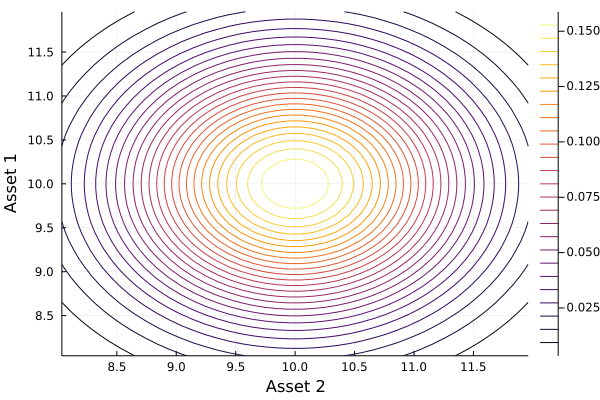
\includegraphics[width=0.9\paperheight]{complexity_files/figure-beamer/unnamed-chunk-2-1} \end{center}

Traditional models of information choice use unimodal joint densities
with good properties. The above is the case used in Kacperczyk et
al.~(2016).
\end{frame}

\begin{frame}{Complexity}
\protect\hypertarget{complexity-2}{}
\begin{center}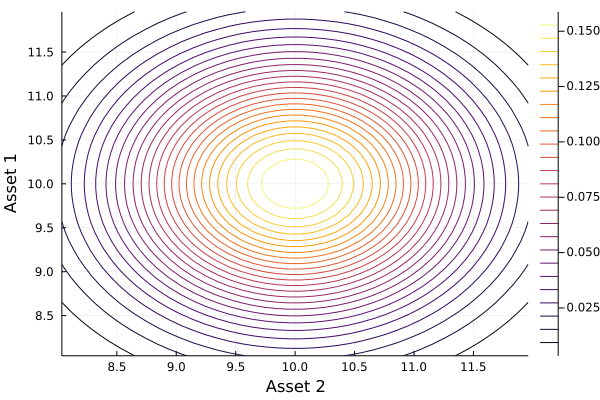
\includegraphics[width=0.9\paperheight]{complexity_files/figure-beamer/unnamed-chunk-3-1} \end{center}

Gaussian variables are the highest entropy distribution for a given mean
and standard deviation, meaning they are the least ``structured''.
\end{frame}

\begin{frame}{Complexity}
\protect\hypertarget{complexity-3}{}
\begin{center}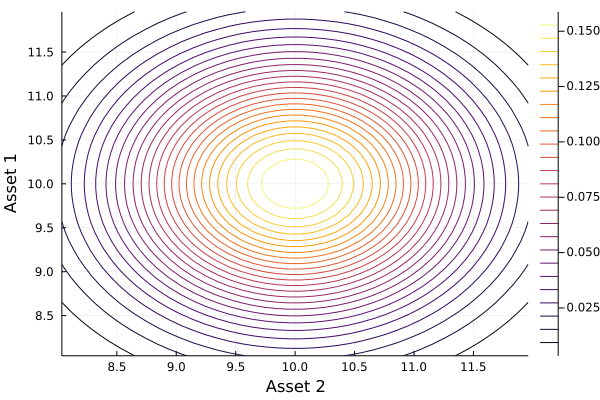
\includegraphics[width=0.9\paperheight]{complexity_files/figure-beamer/unnamed-chunk-4-1} \end{center}

Less structure means a boring blob of investors are generally happy with
any minimum-variance outcome!
\end{frame}

\begin{frame}{Complexity}
\protect\hypertarget{complexity-4}{}
\begin{center}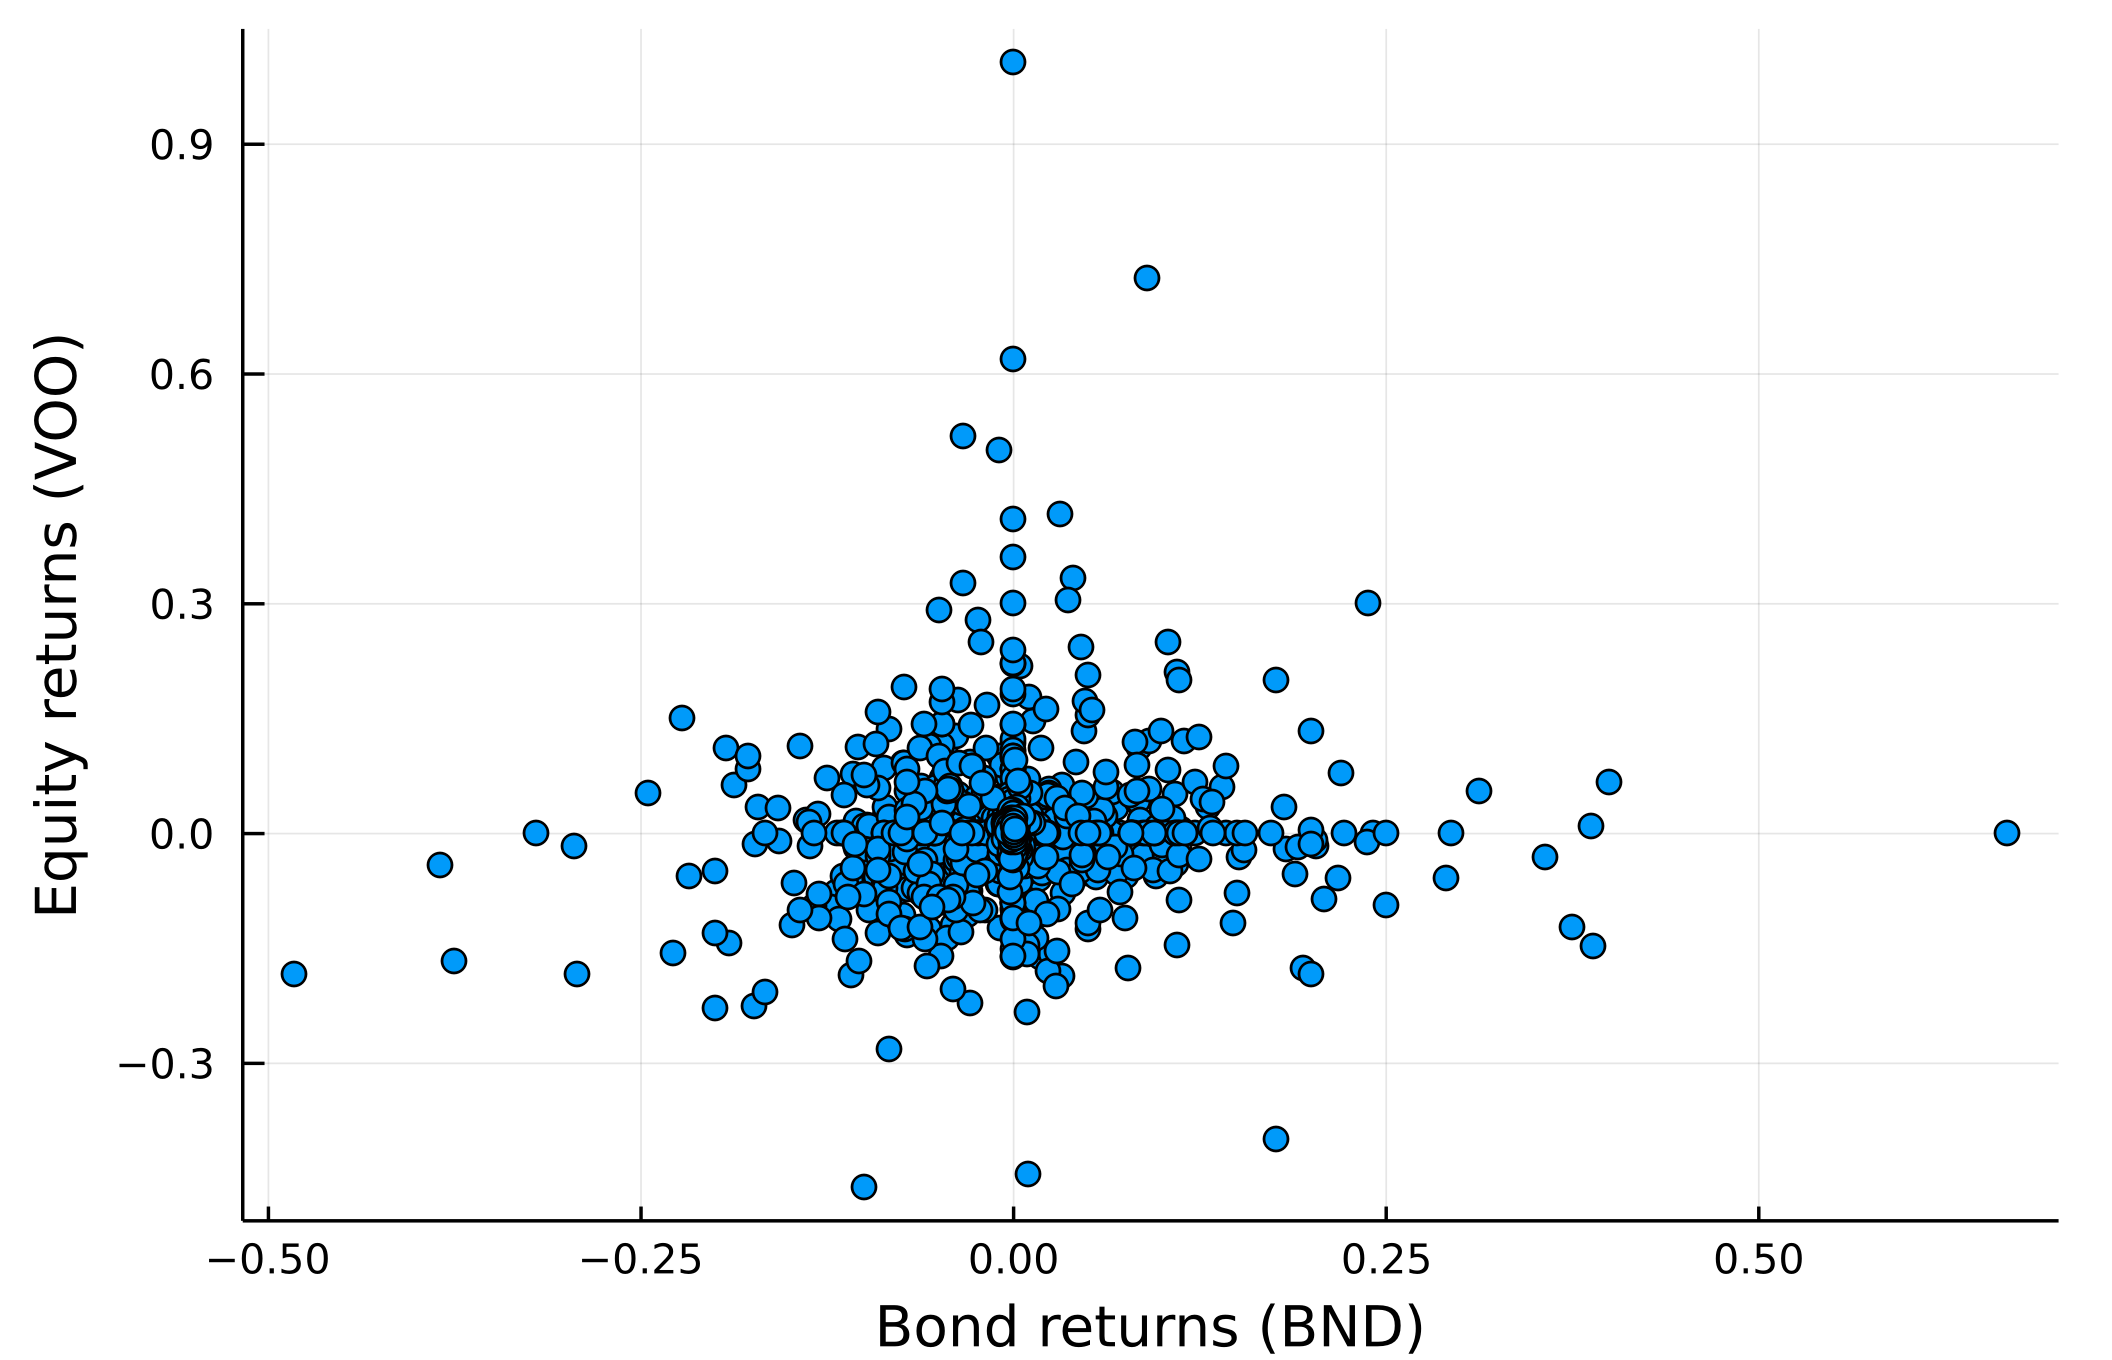
\includegraphics[width=0.9\paperheight]{complexity_files/figure-beamer/unnamed-chunk-5-1} \end{center}

What if payoffs were more ``complicated''? Pictured is the daily
bond/equity observed returns from 2000-2021.
\end{frame}

\begin{frame}{Some hypothetical payoff densities}
\protect\hypertarget{some-hypothetical-payoff-densities}{}
\begin{center}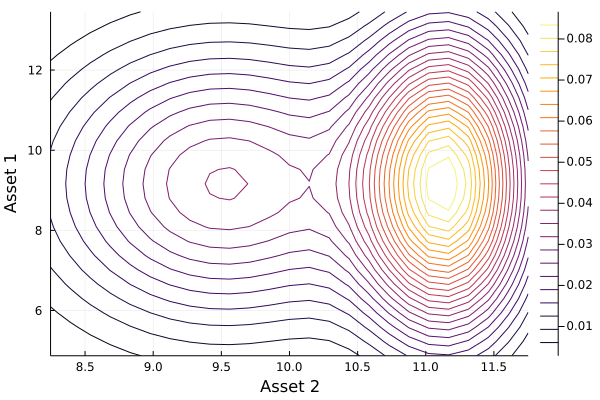
\includegraphics[width=0.8\paperheight]{complexity_files/figure-beamer/unnamed-chunk-6-1} \end{center}
\end{frame}

\begin{frame}{Some hypothetical payoff densities}
\protect\hypertarget{some-hypothetical-payoff-densities-1}{}
\begin{center}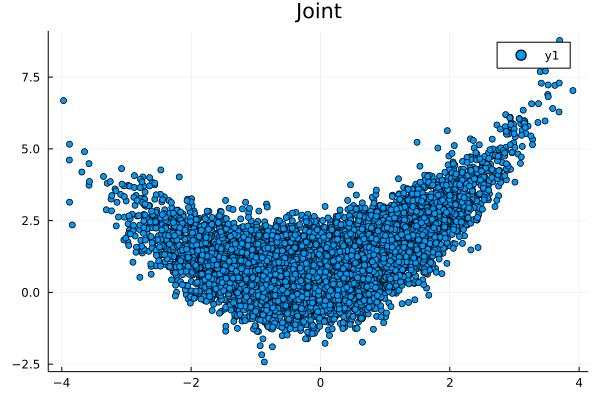
\includegraphics[width=0.8\paperheight]{complexity_files/figure-beamer/unnamed-chunk-7-1} \end{center}
\end{frame}

\begin{frame}{The banana}
\protect\hypertarget{the-banana}{}
\begin{center}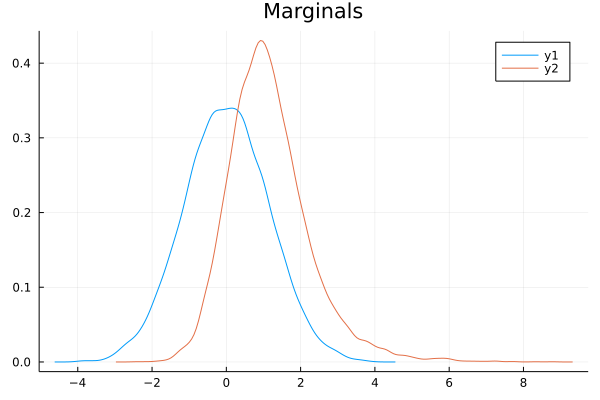
\includegraphics[width=0.5\paperheight]{complexity_files/figure-beamer/unnamed-chunk-8-1} \end{center}
\end{frame}

\begin{frame}{The banana's marginal densities}
\protect\hypertarget{the-bananas-marginal-densities}{}
\begin{center}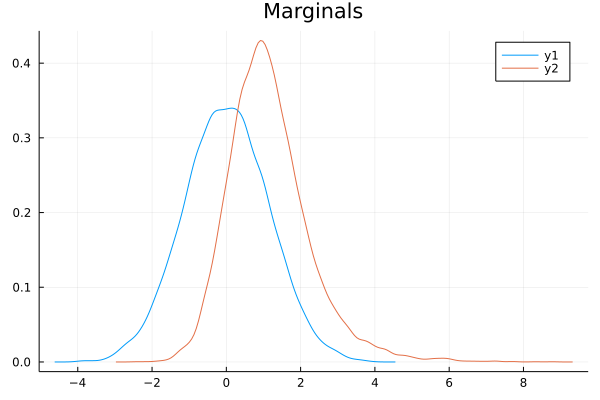
\includegraphics[width=0.5\paperheight]{complexity_files/figure-beamer/unnamed-chunk-9-1} \end{center}

Note that the marginals look pretty close to actual stock return
densities, even though the joint distribution is strange.
\end{frame}

\begin{frame}{The banana takeaway}
\protect\hypertarget{the-banana-takeaway}{}
\begin{center}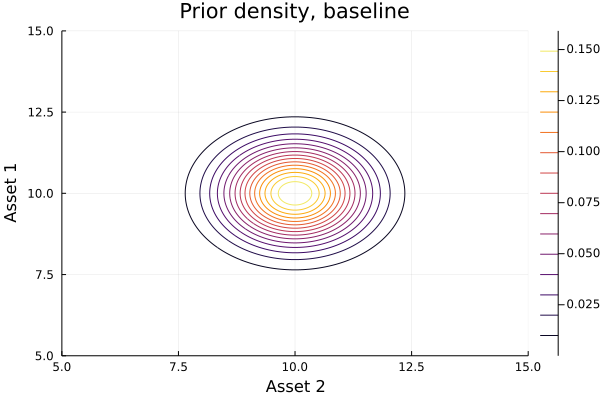
\includegraphics[width=0.5\paperheight]{complexity_files/figure-beamer/unnamed-chunk-10-1} \end{center}

\textbf{How do you allocate attention} if you know you have a
complicated joint density?
\end{frame}

\hypertarget{the-framework}{%
\section{The framework}\label{the-framework}}

\begin{frame}{The framework}
\protect\hypertarget{the-framework-1}{}
I mostly follow Kacperczyk et al.~(2016), which adds attention to the
multiasset noisy rational expectations model of Admati (1985).
\end{frame}

\begin{frame}{States of the economy}
\protect\hypertarget{states-of-the-economy}{}
The economy has a \emph{state}, denoted with \(s\). A \emph{state}
describes the mean and variance of the payoffs in that state,
i.e.~\(\mu_H\) is the mean payoff in the good state, while \(\mu_L\) is
the mean payoff in the bad state.

Investors do not observe the state but must infer it.
\end{frame}

\begin{frame}{States of the economy}
\protect\hypertarget{states-of-the-economy-1}{}
The density function for the state is:

\[
P(s) = \begin{cases}
    \pi & \text{ if } s = H \\
    1-\pi & \text{ if } s = L \\
\end{cases}
\]
\end{frame}

\begin{frame}{The assets}
\protect\hypertarget{the-assets}{}
We have \(n\) assets that have payoffs

\[
f = \mu_s + \epsilon
\]

where

\begin{align}
    f_i &= \mu_{i,s} + z_i\\
    z &\mid s = [z_1,z_2, \dots, z_n]' \sim \mathcal{N}(0, \Sigma_s) \\
    f &\mid s \sim \mathcal{N}(\mu_{s}, \Sigma_s)
\end{align}
\end{frame}

\begin{frame}{What is this density?}
\protect\hypertarget{what-is-this-density}{}
Formally, this is what is known as a \blue{Gaussian mixture model}.
Gaussian mixture models can be used to approximate any joint
density\footnote{If you have ever used kernel density estimation, this is technically what is happening behind the scenes.}

The density function is

\[
P(f) \sim \pi \mathcal{N}(f \mid \mu_H, \Sigma_H) + (1-\pi) \mathcal{N} (f \mid \mu_L, \Sigma_L)
\]
\end{frame}

\begin{frame}{Asset supply}
\protect\hypertarget{asset-supply}{}
The \(n\) assets have an uncertain supply. Sometimes noise traders show
up to trade, so the traders cannot perfectly forecast how many shares
need to be net bought or sold.

Denote this stochastic supply with

\[
x \sim \mathcal{N}(\overline x, \Sigma_x)
\]
\end{frame}

\begin{frame}{Timing}
\protect\hypertarget{timing}{}
\begin{enumerate}
\tightlist
\item
  Investors allocate \red{attention} and then observe signals, if they
  are informed.
\item
  Investors choose \red{asset portfolios} and the market clears.
\item
  Everyone receives the final payoff \(q'_j f\).
\end{enumerate}
\end{frame}

\begin{frame}{The investors}
\protect\hypertarget{the-investors}{}
There is a unit mass of investors \(j \in [0,1]\). Each investor has
CARA utility of the form

\[
U_{j2} = E_j[\exp{-\rho W_j}]
\]

for terminal wealth

\[
W_j = r W_0 + q'_j (f - pr)
\]

where \(W_0\) is initial wealth, \(q'_j\) is the asset quantity
purchased, \(f\) is the realized stochastic payoffs, and \(p\) is the
asset price vector. The risk-free rate of \(r\) is normalized to 1 to
reduce notation.
\end{frame}

\begin{frame}{Private signals}
\protect\hypertarget{private-signals}{}
Some portion of investors receive \red{private signals} of the true
payoff \(f\). Their signals take the form

\begin{align}
    \eta_j &\sim \mathcal{N}(f, \Sigma_{\eta,j}), \\
    \text{ or } \eta_j &= f + \epsilon_j, \quad \epsilon_j \sim \mathcal{N}(0, \Sigma_{\eta_j})
\end{align}
\end{frame}

\begin{frame}{Private signals}
\protect\hypertarget{private-signals-1}{}
Investors can control how precise this signal is at the beginning of the
game by allocating attention.

\[
\Sigma_{\eta_j} = \begin{bmatrix}
  K_{1j}^{-1} & 0 & \dots & 0 \\
  0 & K_{2j}^{-1} & \dots & 0 \\
  0 & 0 & \ddots & 0 \\
  0 & 0 & 0 & K_{nj}^{-1} \\
\end{bmatrix}
\]

Subject to the constraints that \(K_ij \ge 0\) (no forgetting) and
\(\sum K_ij \le K\) (finite attention).
\end{frame}

\begin{frame}{The information choice problem}
\protect\hypertarget{the-information-choice-problem}{}
The information choice problem is the one I want to focus on, but it's
hard to get to!

Ultimately, I want to know the gradients of the attention allocation
function

\[
\Sigma^*_{\eta_j}(\pi, \mu_H, \mu_L, \Sigma_H, \Sigma_L)
\]

with respect to the prior payoff parameters.
\end{frame}

\begin{frame}{Portfolio choice}
\protect\hypertarget{portfolio-choice}{}
The portfolio choice problem is quite easy. Assume that investors have
their signals \(\eta_j\) and can see prices \(p\). Then they must
maximize expected terminal utility:

\begin{maxi}
    {q_{j}}{U_{j2} = E_j[\exp{-\rho W_j} \mid \eta_j, p]}
    {\label{eq:learning-opt}}{}
    \addConstraint{W_j }{= r W_0 + q'_j (f - pr)}
\end{maxi}
\end{frame}

\begin{frame}{Portfolio choice}
\protect\hypertarget{portfolio-choice-1}{}
Solving this yields the (maybe familiar) exact quantity:

\newcommand{\shat}{\hat s_j}
\newcommand{\hShat}{\hat \Sigma_{H,j}}
\newcommand{\lShat}{\hat \Sigma_{L,j}}
\newcommand{\hMhat}{\hat \mu_{H,j}}
\newcommand{\lMhat}{\hat \mu_{L,j}}

\begin{align}
    q_j = \frac{1}{\rho}\big(\hat s_j\hat \Sigma_{H,j}+ (1-\hat s_j) \hat \Sigma_{L,j}\big)^{-1}\big(\hat s_j\hat \mu_{H,j}+ (1-\hat s_j) \hat \mu_{L,j}\big)
\end{align}

for posterior state beliefs after observing \(p\) and \(\eta_j\).
\end{frame}

\begin{frame}{Prices}
\protect\hypertarget{prices}{}
Prices are the tricky bit in this economy. In other models, you can
conjecture a linear price as a function of the true payoffs \(f\) and
the supply \(x\):

\[
p = A + B f + C x
\]

Kacperczyk et al.~(2016) and others have exact forms for these matrices.
\end{frame}

\begin{frame}{Prices}
\protect\hypertarget{prices-1}{}
I don't! It's been very difficult even with a simple density to get
closed form prices, partly because everyone's posterior beliefs about
the state (\(\hat s_j\)) move around with \(f\).

This means that prices \(p\) are linear in \(f\) and \(x\), but the
parameters \(A\), \(B\), and \(C\) are non-linear functions of \(f\) and
\(x\).

Tricky!
\end{frame}

\begin{frame}{Solving for prices numerically}
\protect\hypertarget{solving-for-prices-numerically}{}
I can solve for prices numerically by conjecturing \(A\), \(B\), and
\(C\) such that the market clearing condition is satisfied:

\[
\int_j q_j(p) = x
\]
\end{frame}

\hypertarget{example-economies}{%
\section{Example economies}\label{example-economies}}

\begin{frame}{Four economies}
\protect\hypertarget{four-economies}{}
Two asset economies for easy plotting. I set \(\pi = 1/2\) and \(K=10\)
in all cases.

\begin{table}
\begin{tabular}{ccccc}
  \toprule
  & $\mu_H$ & $\mu_L$ & $\Sigma_H$ & $\Sigma_L$ \\
  \midrule
  1 & $[10,10]$ & $[10,10]$ & $I$ & $I$ \\
  2 & $[10,12]$ & $[10,8]$ & $I$ & $I$ \\
  3 & $[10,12]$ & $[10,8]$ & $I$ & $[1, 0; 0, 5]$ \\
  4 & $[10,12]$ & $[10,8]$ & $I$ & $[2, 0.4; 0.4, 2]$ \\
\end{tabular}
\end{table}
\end{frame}

\begin{frame}{Prior payoffs}
\protect\hypertarget{prior-payoffs}{}
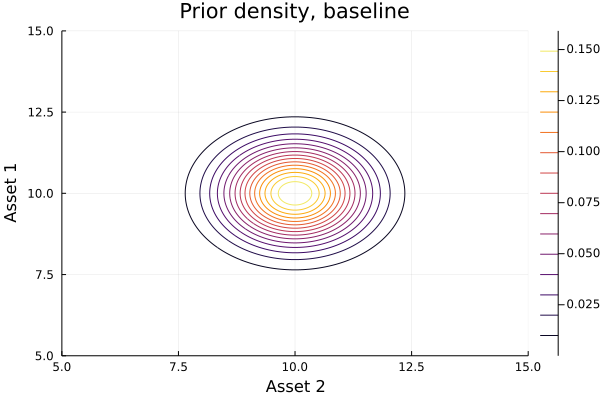
\includegraphics[width=0.5\paperheight]{complexity_files/figure-beamer/unnamed-chunk-11-1}
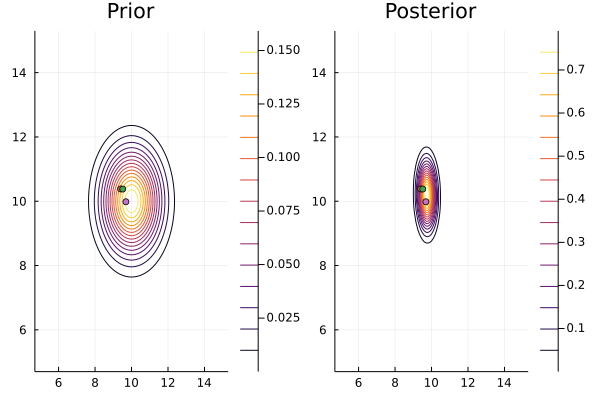
\includegraphics[width=0.5\paperheight]{complexity_files/figure-beamer/unnamed-chunk-11-2}
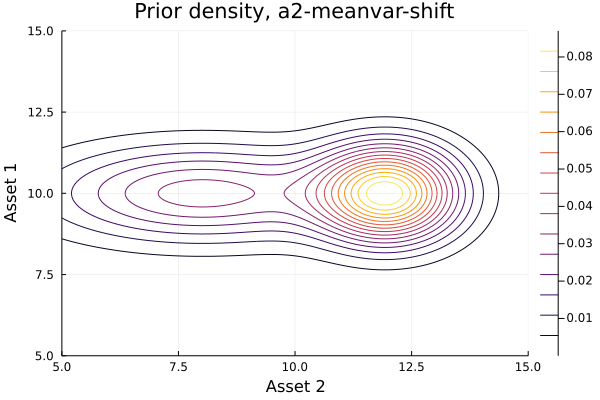
\includegraphics[width=0.5\paperheight]{complexity_files/figure-beamer/unnamed-chunk-11-3}
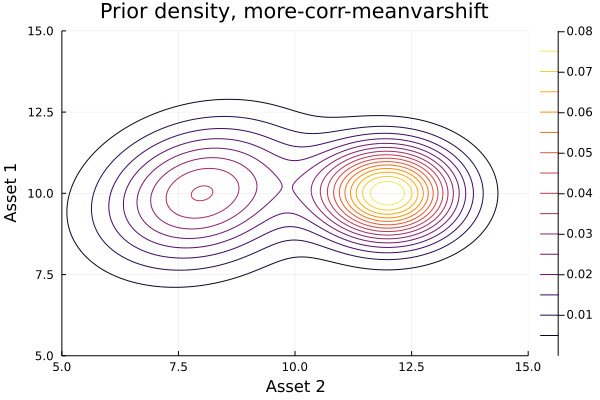
\includegraphics[width=0.5\paperheight]{complexity_files/figure-beamer/unnamed-chunk-11-4}
\end{frame}

\begin{frame}{The investors}
\protect\hypertarget{the-investors-1}{}
To examine how disparate attention impacts each of these economies, I
force half the investors to place \(90\%\) of their attention on asset
1, and the other half to focus \(90\%\) on asset 2.
\end{frame}

\begin{frame}{Baseline (investor posterior)}
\protect\hypertarget{baseline-investor-posterior}{}
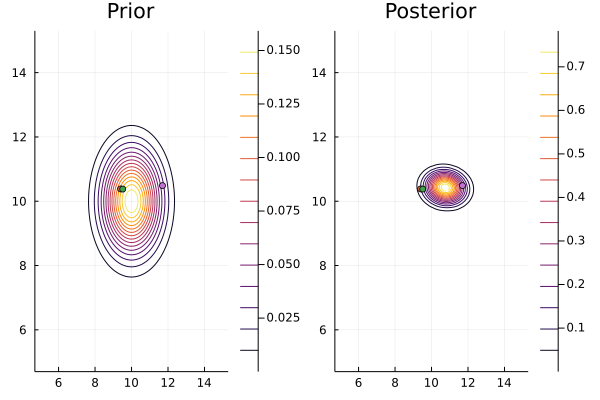
\includegraphics[width=0.4\paperwidth]{complexity_files/figure-beamer/unnamed-chunk-12-1}
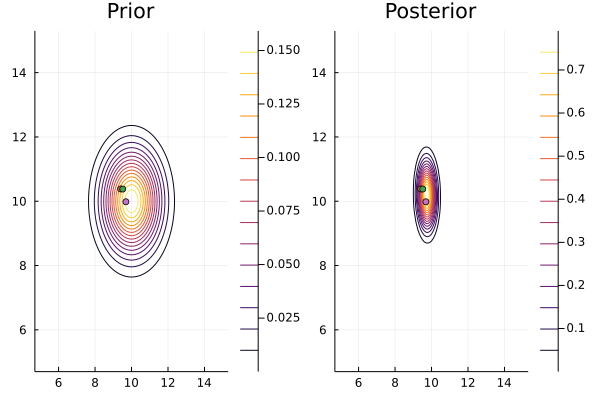
\includegraphics[width=0.4\paperwidth]{complexity_files/figure-beamer/unnamed-chunk-12-2}
\end{frame}

\begin{frame}{Mean shift (investor posterior)}
\protect\hypertarget{mean-shift-investor-posterior}{}
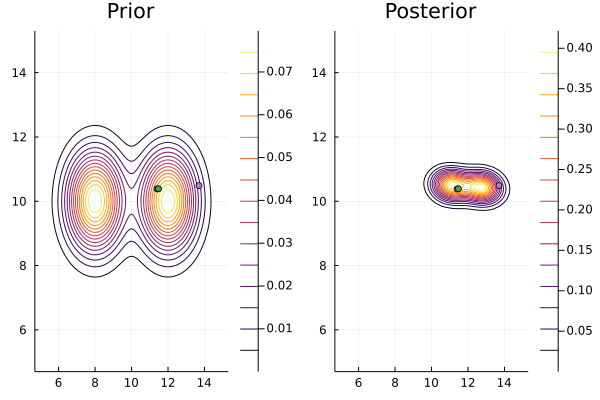
\includegraphics[width=0.4\paperwidth]{complexity_files/figure-beamer/unnamed-chunk-13-1}
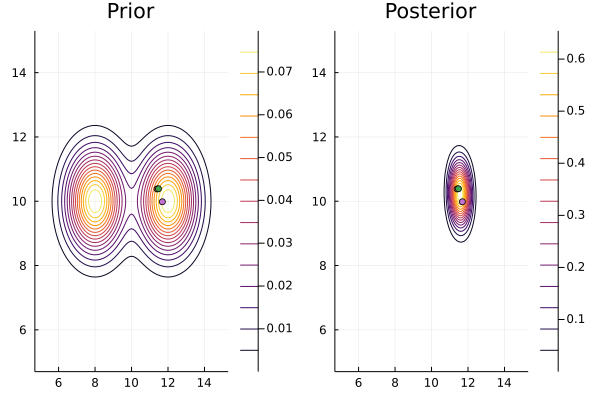
\includegraphics[width=0.4\paperwidth]{complexity_files/figure-beamer/unnamed-chunk-13-2}
\end{frame}

\begin{frame}{Mean and variance shift (investor posterior)}
\protect\hypertarget{mean-and-variance-shift-investor-posterior}{}
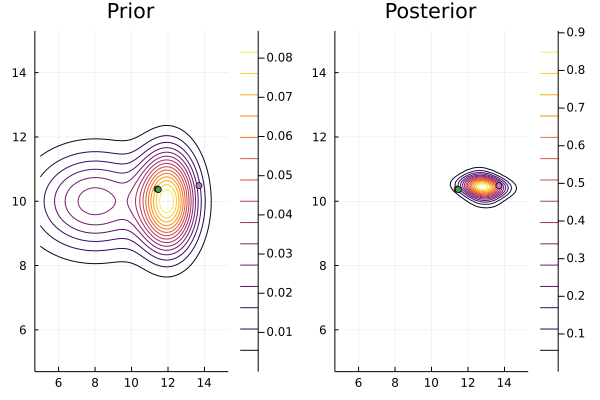
\includegraphics[width=0.4\paperwidth]{complexity_files/figure-beamer/unnamed-chunk-14-1}
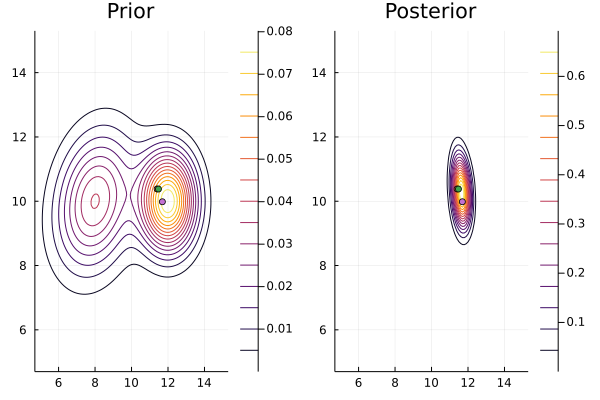
\includegraphics[width=0.4\paperwidth]{complexity_files/figure-beamer/unnamed-chunk-14-2}
\end{frame}

\begin{frame}{Mean, correlation, and variance shift (investor
posterior)}
\protect\hypertarget{mean-correlation-and-variance-shift-investor-posterior}{}
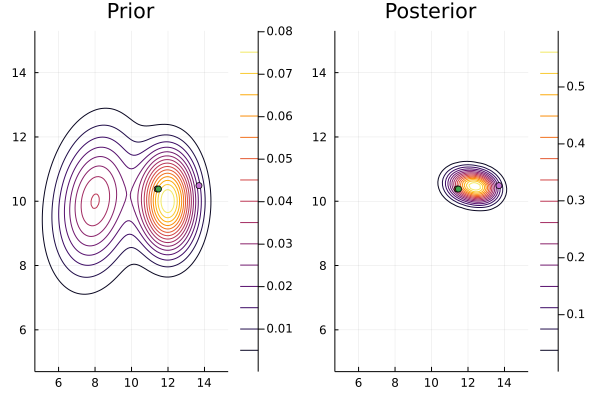
\includegraphics[width=0.4\paperwidth]{complexity_files/figure-beamer/unnamed-chunk-15-1}
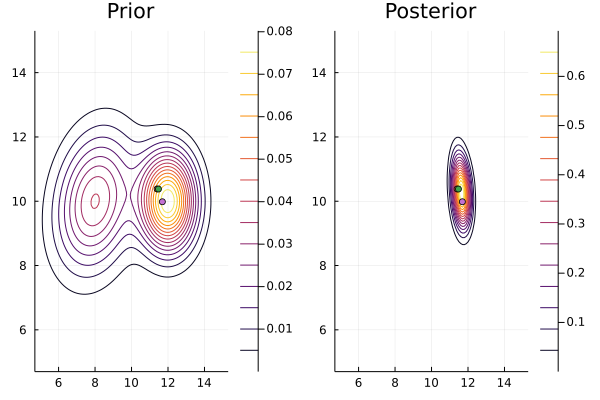
\includegraphics[width=0.4\paperwidth]{complexity_files/figure-beamer/unnamed-chunk-15-2}
\end{frame}

\begin{frame}{What do investors think expected returns are
(\(E[f/p - 1]\))?}
\protect\hypertarget{what-do-investors-think-expected-returns-are-efp---1}{}
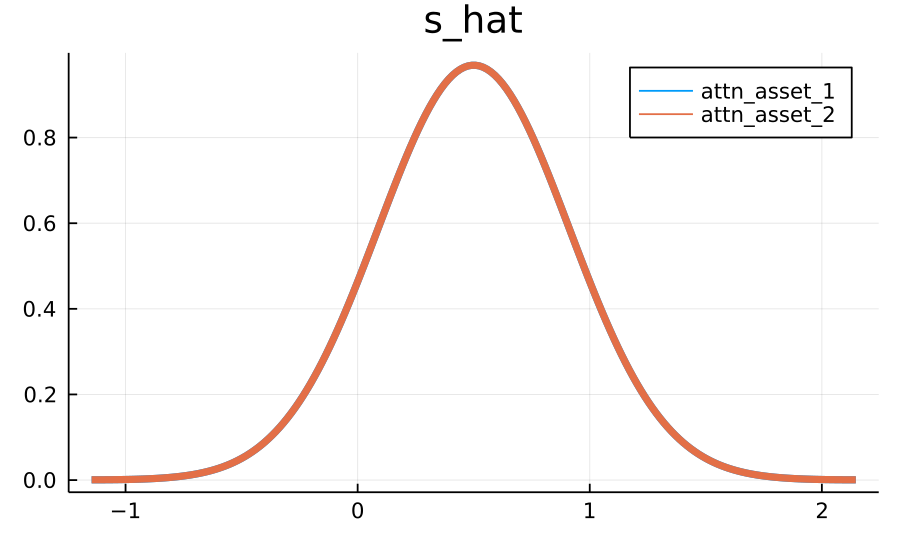
\includegraphics[width=0.4\paperheight]{complexity_files/figure-beamer/unnamed-chunk-16-1}
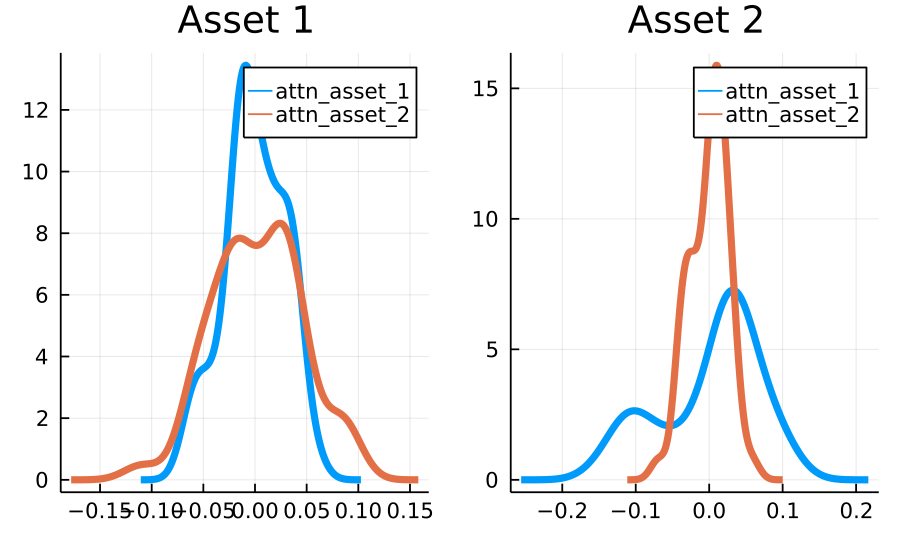
\includegraphics[width=0.4\paperheight]{complexity_files/figure-beamer/unnamed-chunk-16-2}
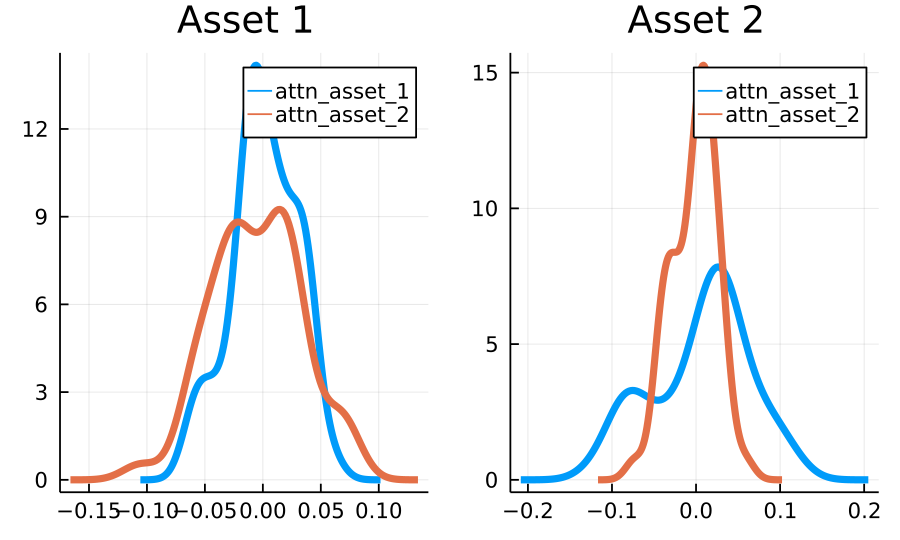
\includegraphics[width=0.4\paperheight]{complexity_files/figure-beamer/unnamed-chunk-16-3}
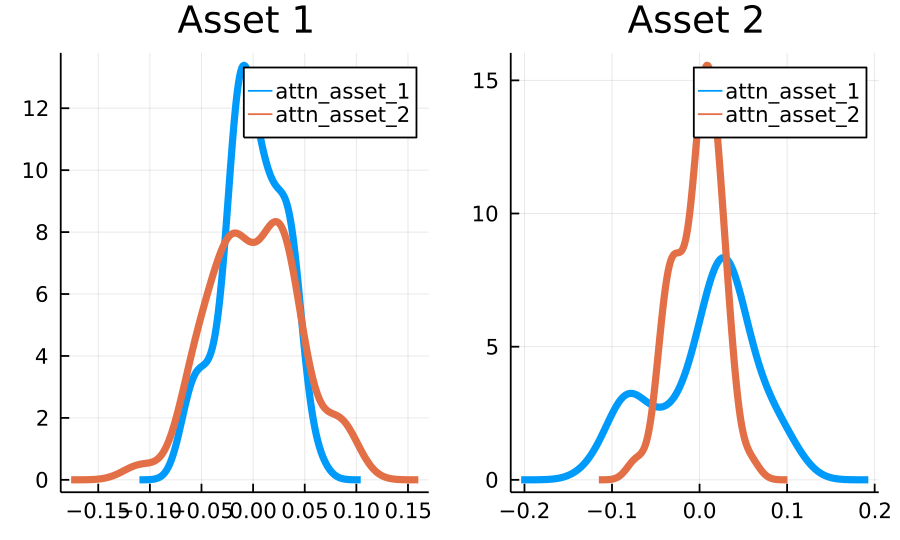
\includegraphics[width=0.4\paperheight]{complexity_files/figure-beamer/unnamed-chunk-16-4}
\end{frame}

\begin{frame}{What do investors think the state is (\(\hat s_j\))?}
\protect\hypertarget{what-do-investors-think-the-state-is-hat-s_j}{}
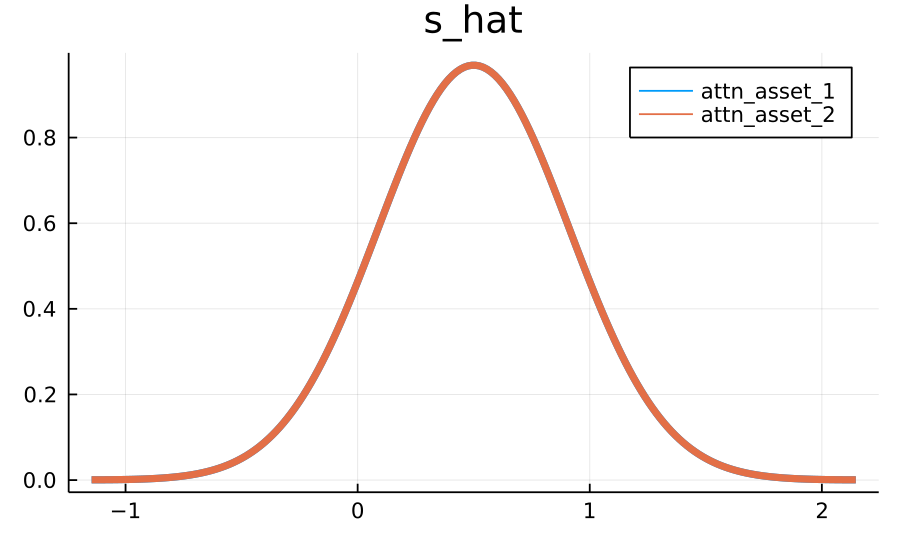
\includegraphics[width=0.4\paperheight]{complexity_files/figure-beamer/unnamed-chunk-17-1}
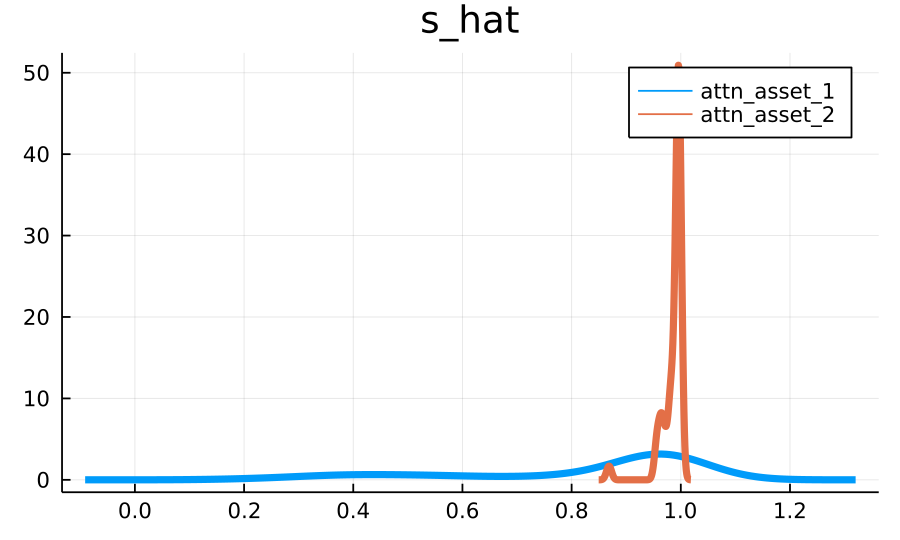
\includegraphics[width=0.4\paperheight]{complexity_files/figure-beamer/unnamed-chunk-17-2}
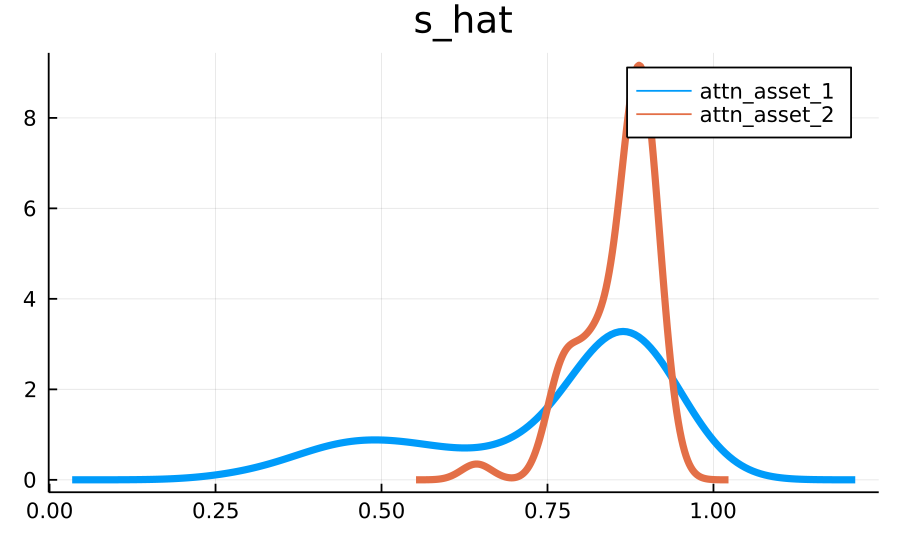
\includegraphics[width=0.4\paperheight]{complexity_files/figure-beamer/unnamed-chunk-17-3}
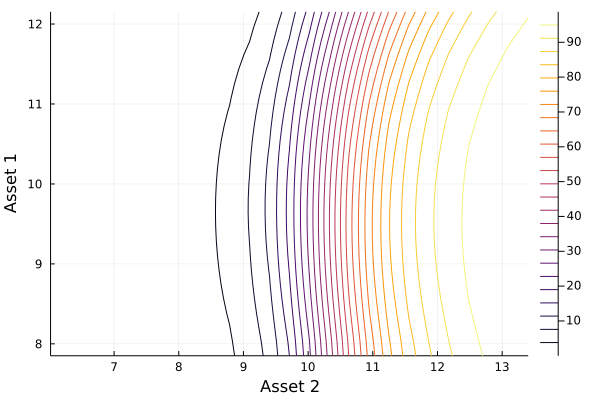
\includegraphics[width=0.4\paperheight]{complexity_files/figure-beamer/unnamed-chunk-17-4}
\end{frame}

\begin{frame}{How much disagreement is there
(\(\text{Var}[\hat s_j]\))?}
\protect\hypertarget{how-much-disagreement-is-there-textvarhat-s_j}{}
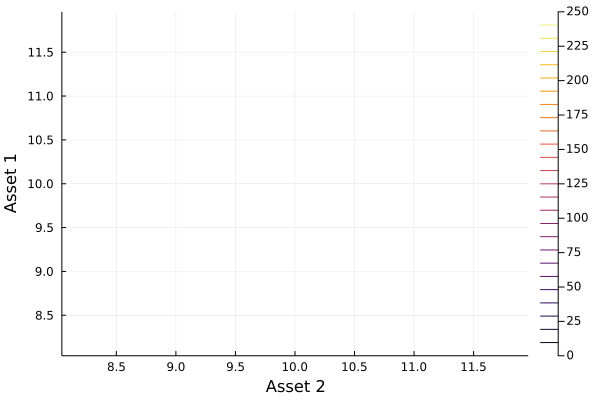
\includegraphics[width=0.4\paperheight]{complexity_files/figure-beamer/unnamed-chunk-18-1}
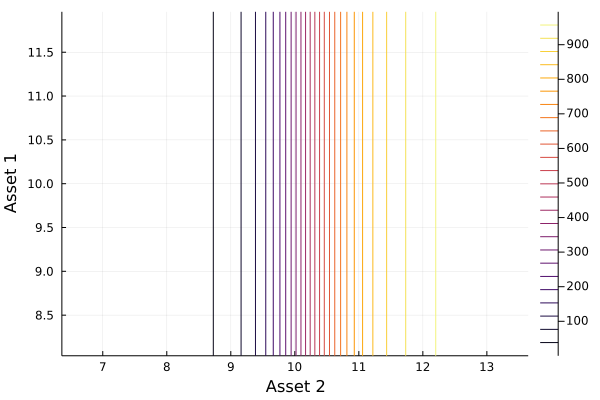
\includegraphics[width=0.4\paperheight]{complexity_files/figure-beamer/unnamed-chunk-18-2}
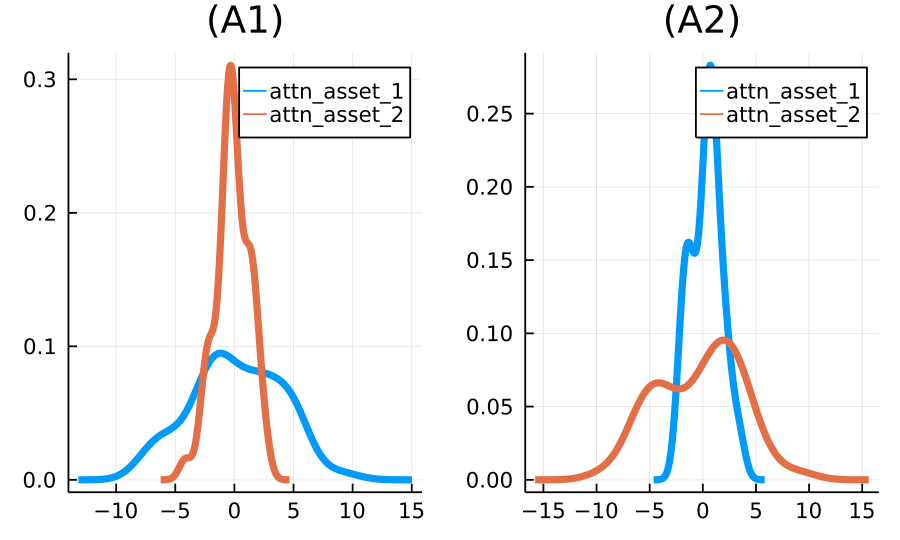
\includegraphics[width=0.4\paperheight]{complexity_files/figure-beamer/unnamed-chunk-18-3}
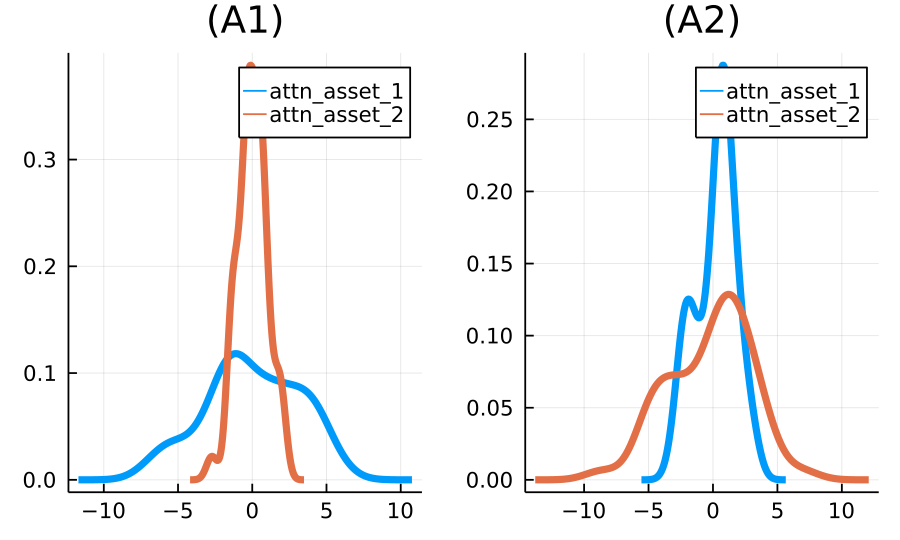
\includegraphics[width=0.4\paperheight]{complexity_files/figure-beamer/unnamed-chunk-18-4}
\end{frame}

\begin{frame}{What do investors buy or sell (\(q_j^*\))?}
\protect\hypertarget{what-do-investors-buy-or-sell-q_j}{}
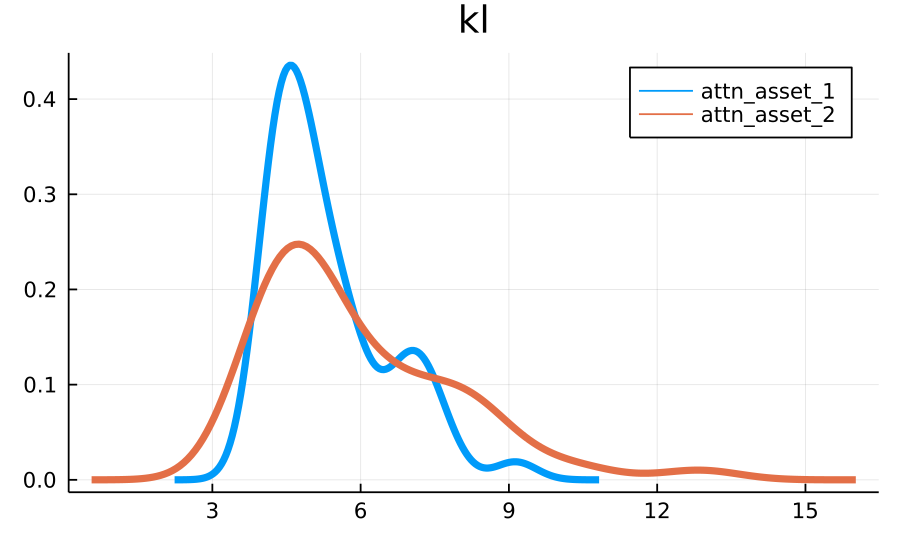
\includegraphics[width=0.4\paperwidth]{complexity_files/figure-beamer/unnamed-chunk-19-1}
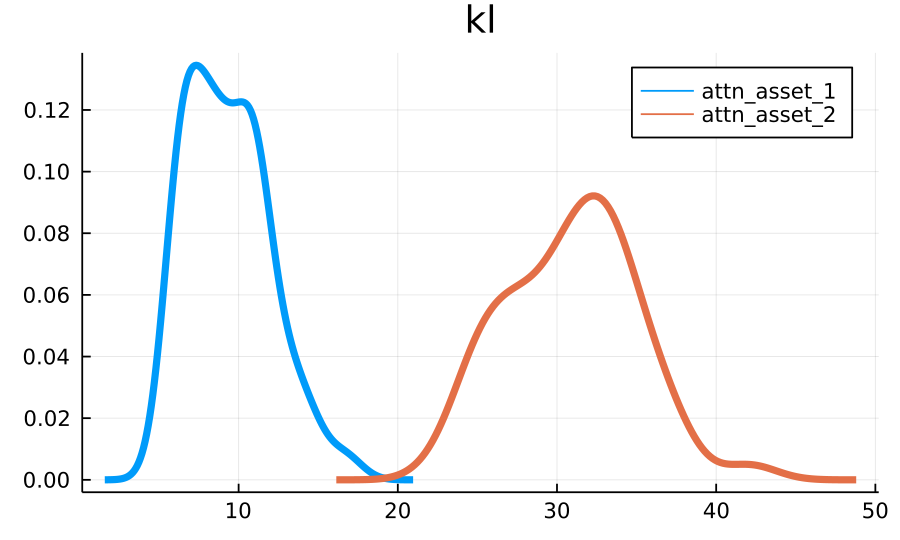
\includegraphics[width=0.4\paperwidth]{complexity_files/figure-beamer/unnamed-chunk-19-2}
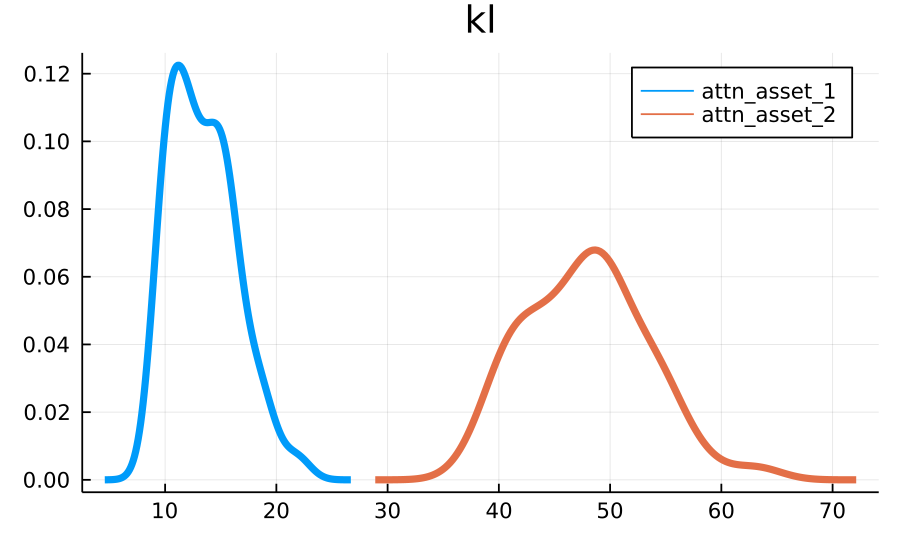
\includegraphics[width=0.4\paperwidth]{complexity_files/figure-beamer/unnamed-chunk-19-3}
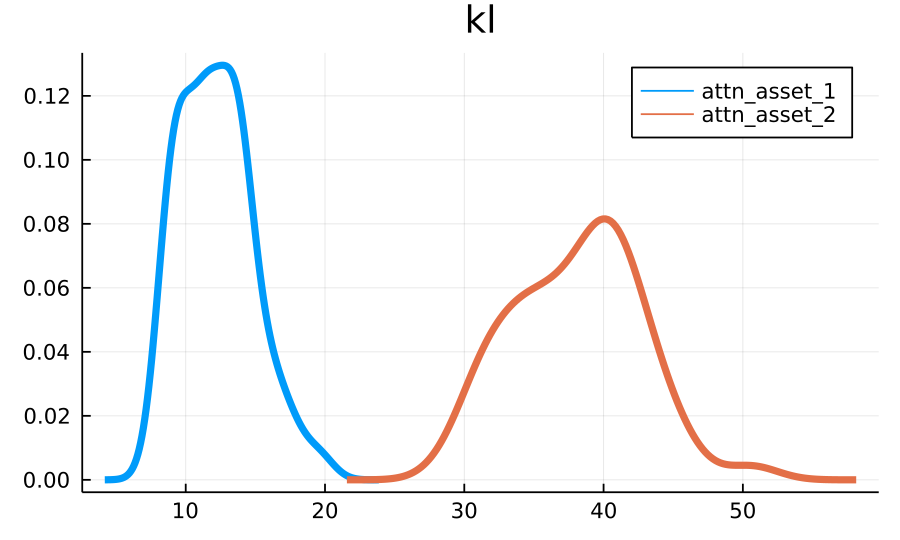
\includegraphics[width=0.4\paperwidth]{complexity_files/figure-beamer/unnamed-chunk-19-4}
\end{frame}

\begin{frame}{Who learns the most (\(KL(\hat f_j \mid\mid f)\))?}
\protect\hypertarget{who-learns-the-most-klhat-f_j-midmid-f}{}
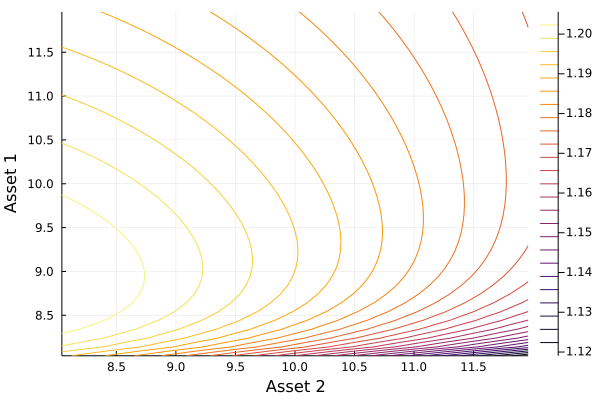
\includegraphics[width=0.4\paperheight]{complexity_files/figure-beamer/unnamed-chunk-20-1}
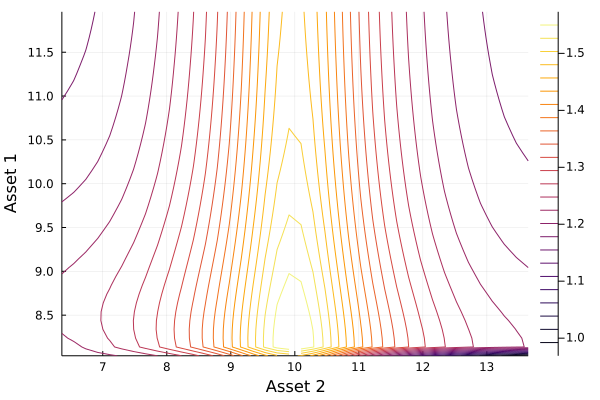
\includegraphics[width=0.4\paperheight]{complexity_files/figure-beamer/unnamed-chunk-20-2}
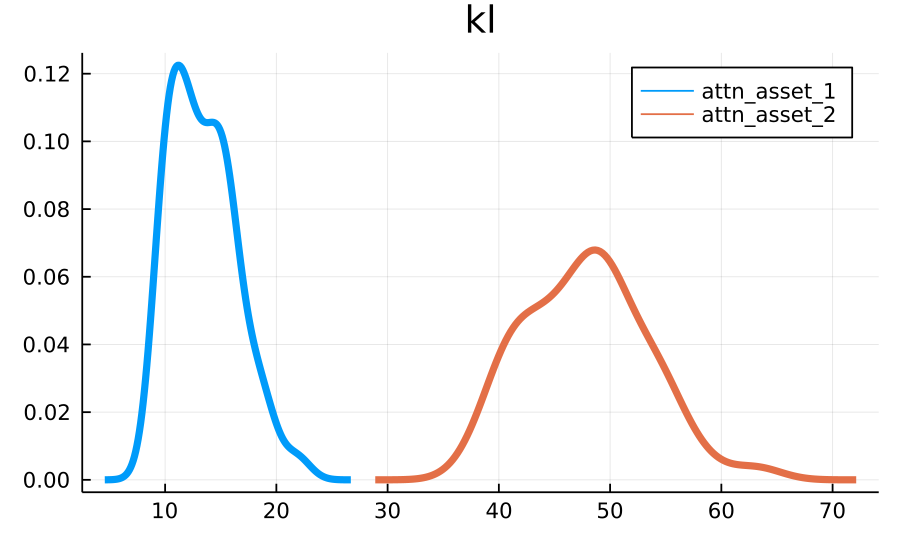
\includegraphics[width=0.4\paperheight]{complexity_files/figure-beamer/unnamed-chunk-20-3}
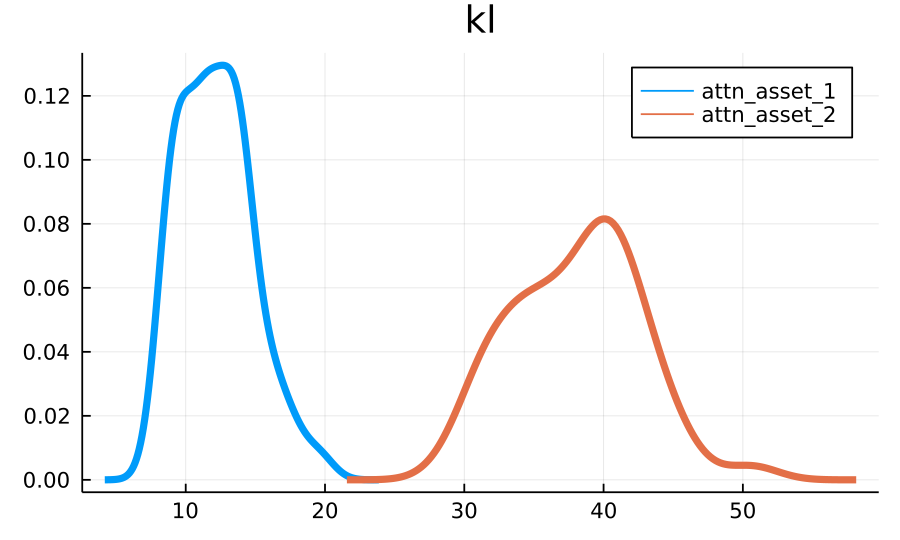
\includegraphics[width=0.4\paperheight]{complexity_files/figure-beamer/unnamed-chunk-20-4}
\end{frame}

\begin{frame}{In what states are investors the most uncertain
(\(\hat H(\hat f_j \mid\mid f)\))?}
\protect\hypertarget{in-what-states-are-investors-the-most-uncertain-hat-hhat-f_j-midmid-f}{}
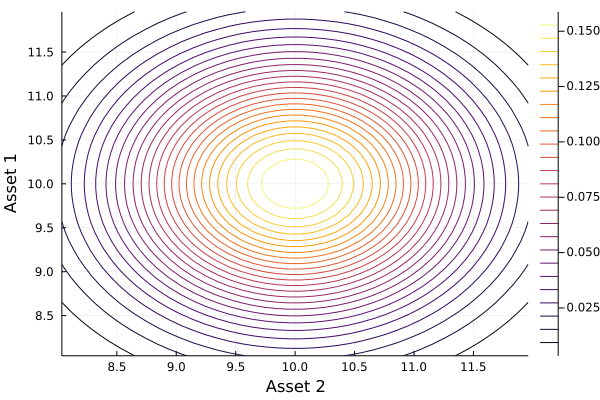
\includegraphics[width=0.4\paperheight]{complexity_files/figure-beamer/unnamed-chunk-21-1}
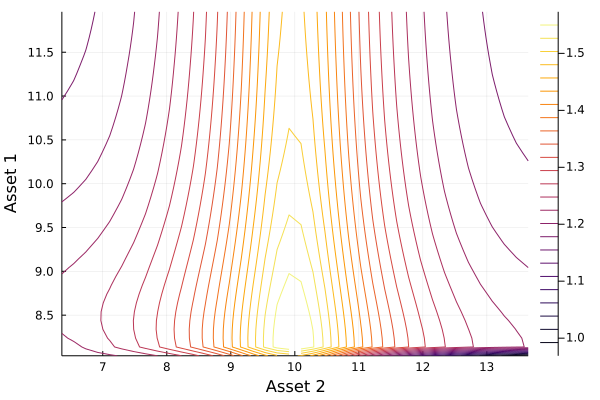
\includegraphics[width=0.4\paperheight]{complexity_files/figure-beamer/unnamed-chunk-21-2}
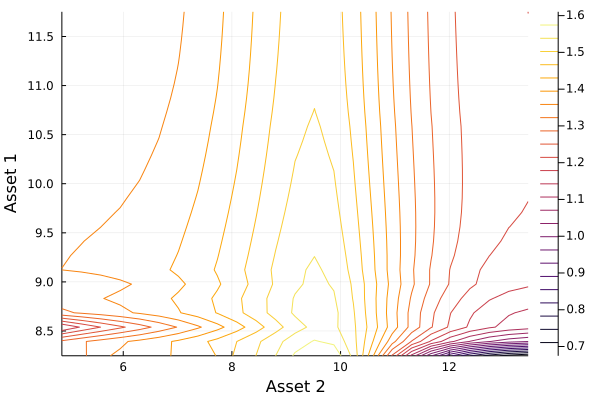
\includegraphics[width=0.4\paperheight]{complexity_files/figure-beamer/unnamed-chunk-21-3}
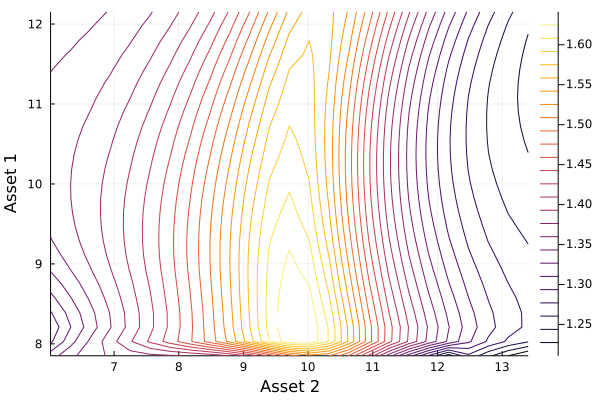
\includegraphics[width=0.4\paperheight]{complexity_files/figure-beamer/unnamed-chunk-21-4}
\end{frame}

\hypertarget{prices-2}{%
\section{Prices}\label{prices-2}}

\begin{frame}{Prices}
\protect\hypertarget{prices-3}{}
My estimation procedure estimates the matrices \(A\), \(B\), and \(C\):

\[
p = A + B f + C x
\]

Since I do not (yet) have a closed form expression for this, I form a
\(50 \times 50\) grid of possible draws of the payoffs \(f\), fixing
supply \(x = \overline x\).

For each \(f\), I calculate the equilibrium conditions and store them.
This lets me plot out the approximate pricing function!
\end{frame}

\begin{frame}{}
\protect\hypertarget{section}{}
\begin{center}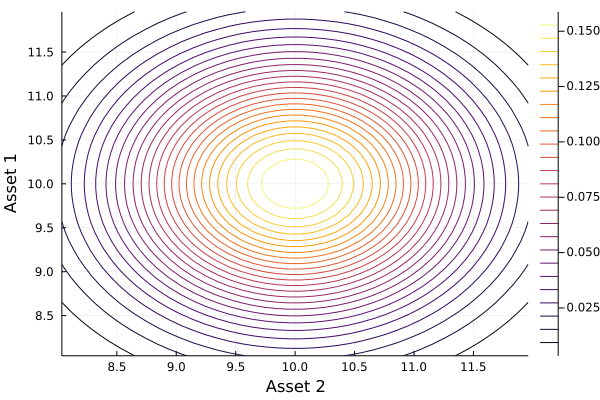
\includegraphics[width=0.95\paperheight]{complexity_files/figure-beamer/unnamed-chunk-22-1} \end{center}
\end{frame}

\begin{frame}{}
\protect\hypertarget{section-1}{}
\begin{center}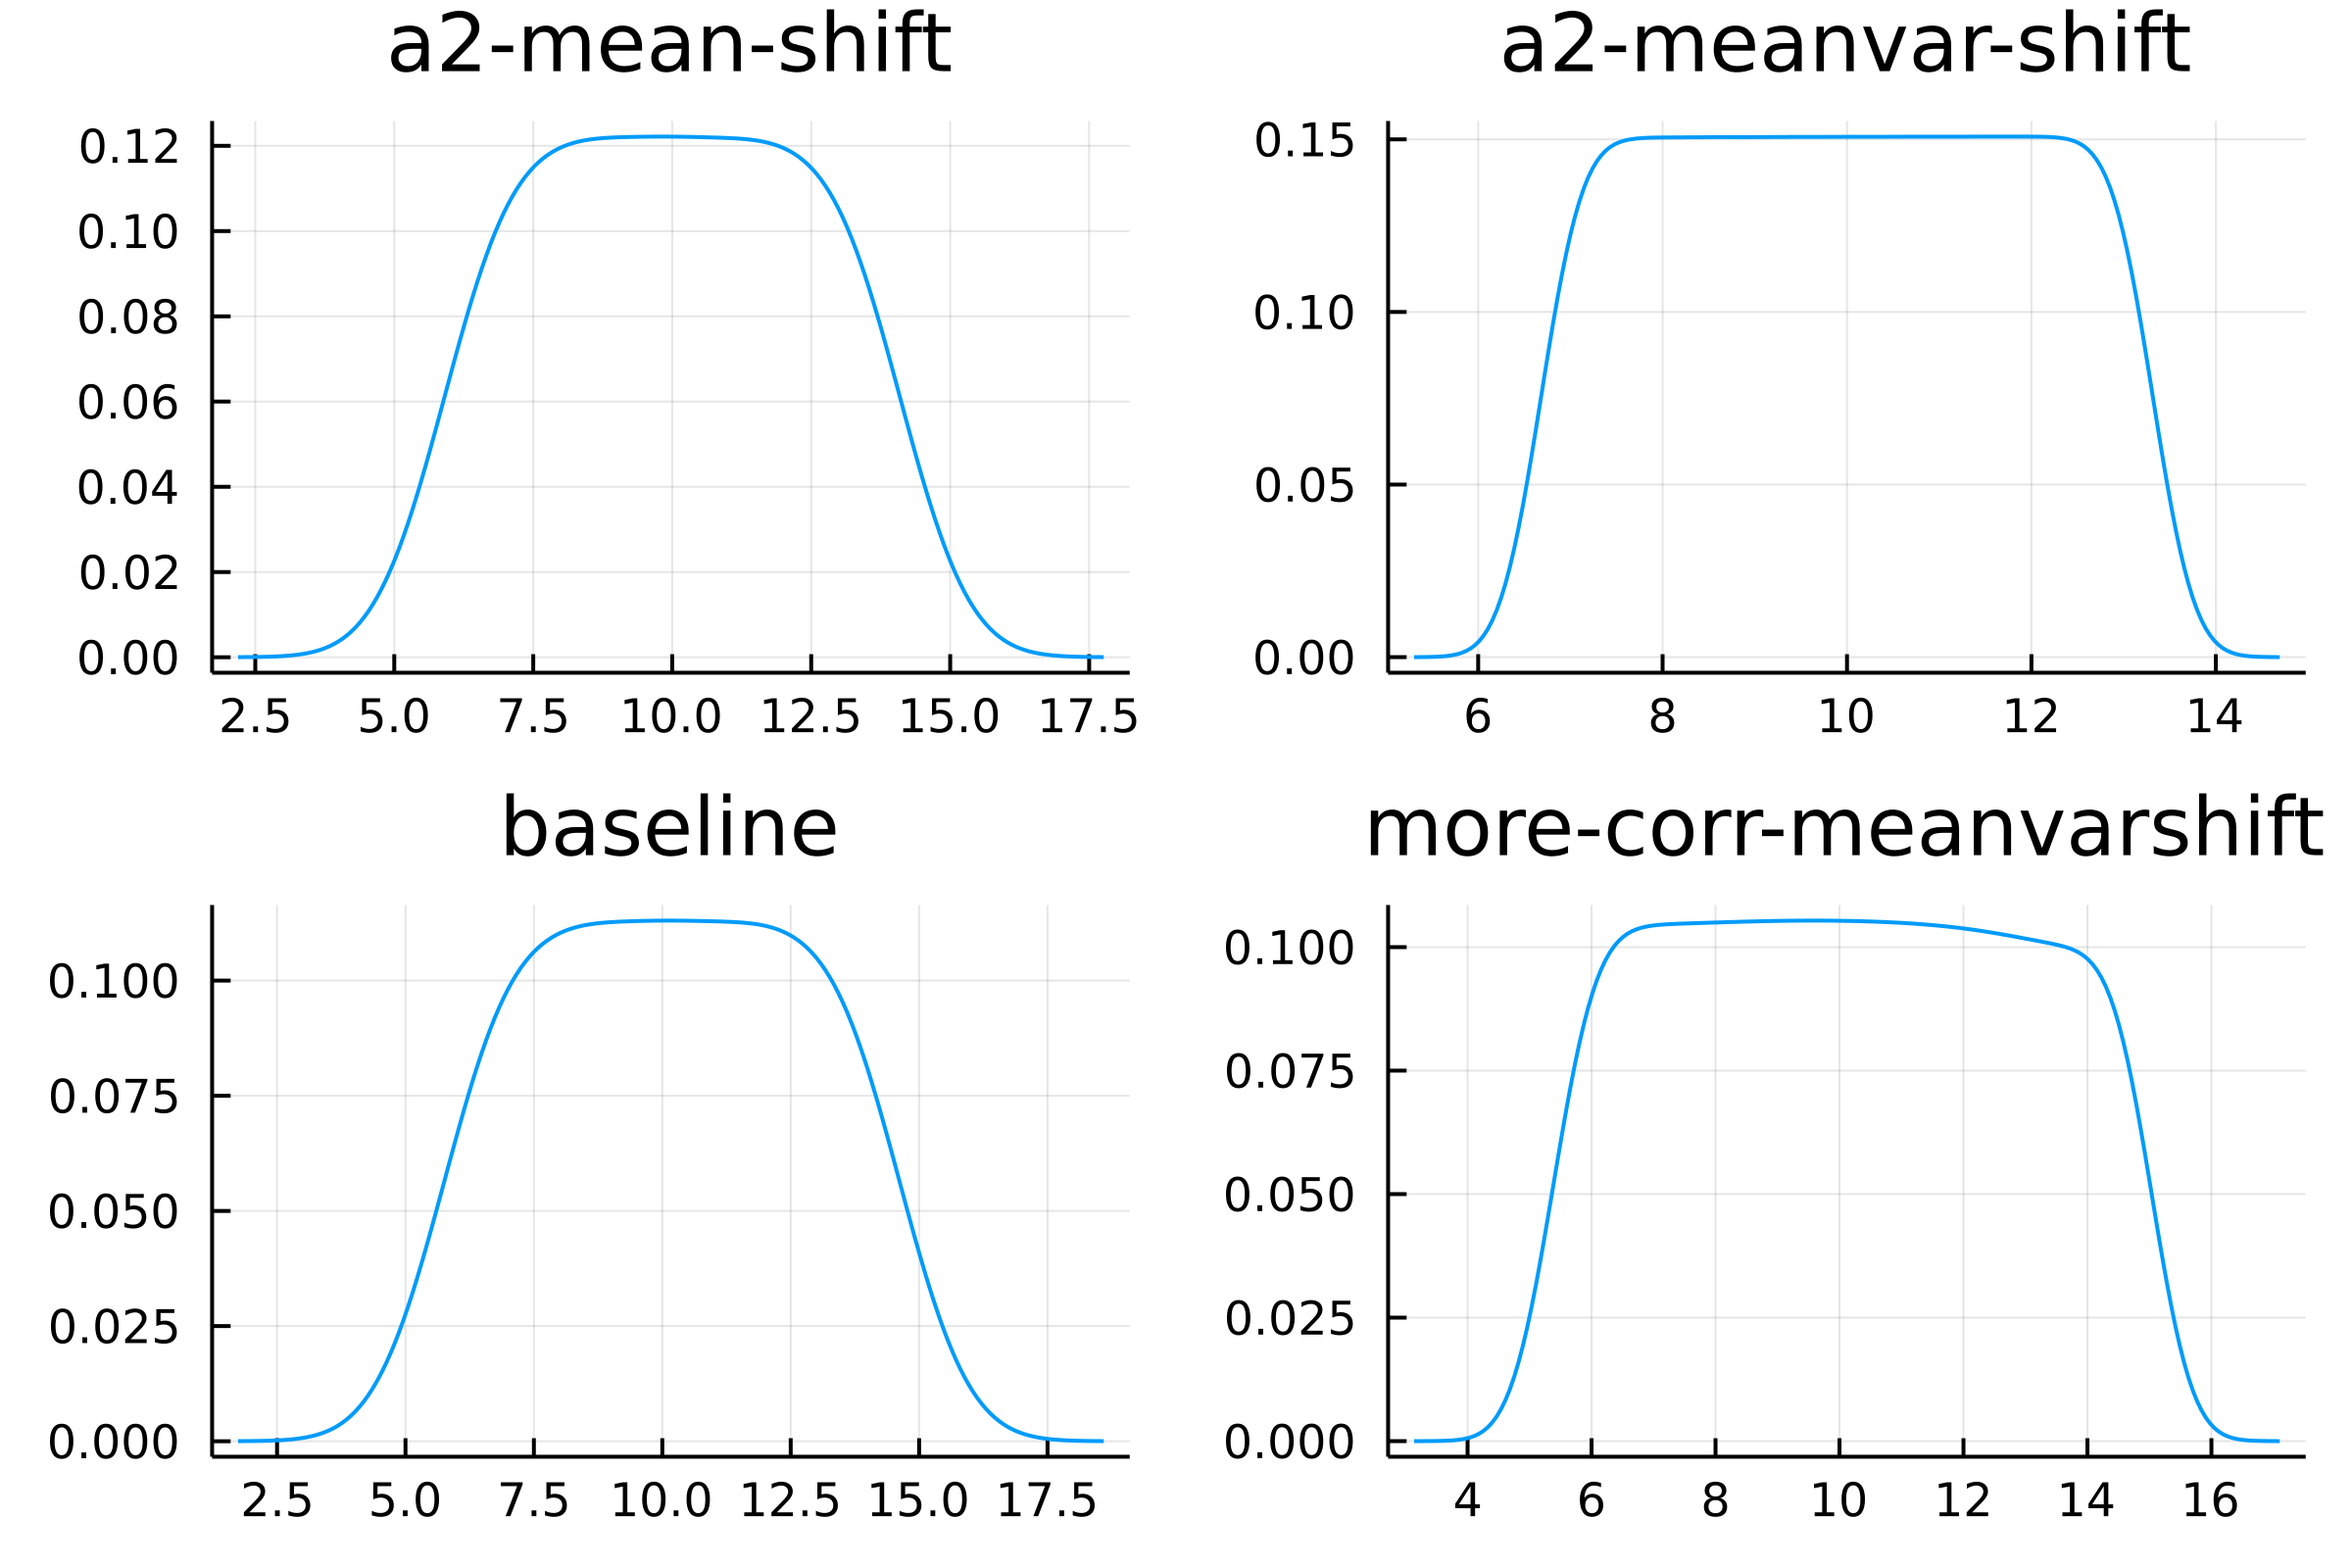
\includegraphics[width=0.95\paperheight]{complexity_files/figure-beamer/unnamed-chunk-23-1} \end{center}
\end{frame}

\begin{frame}{}
\protect\hypertarget{section-2}{}
\begin{center}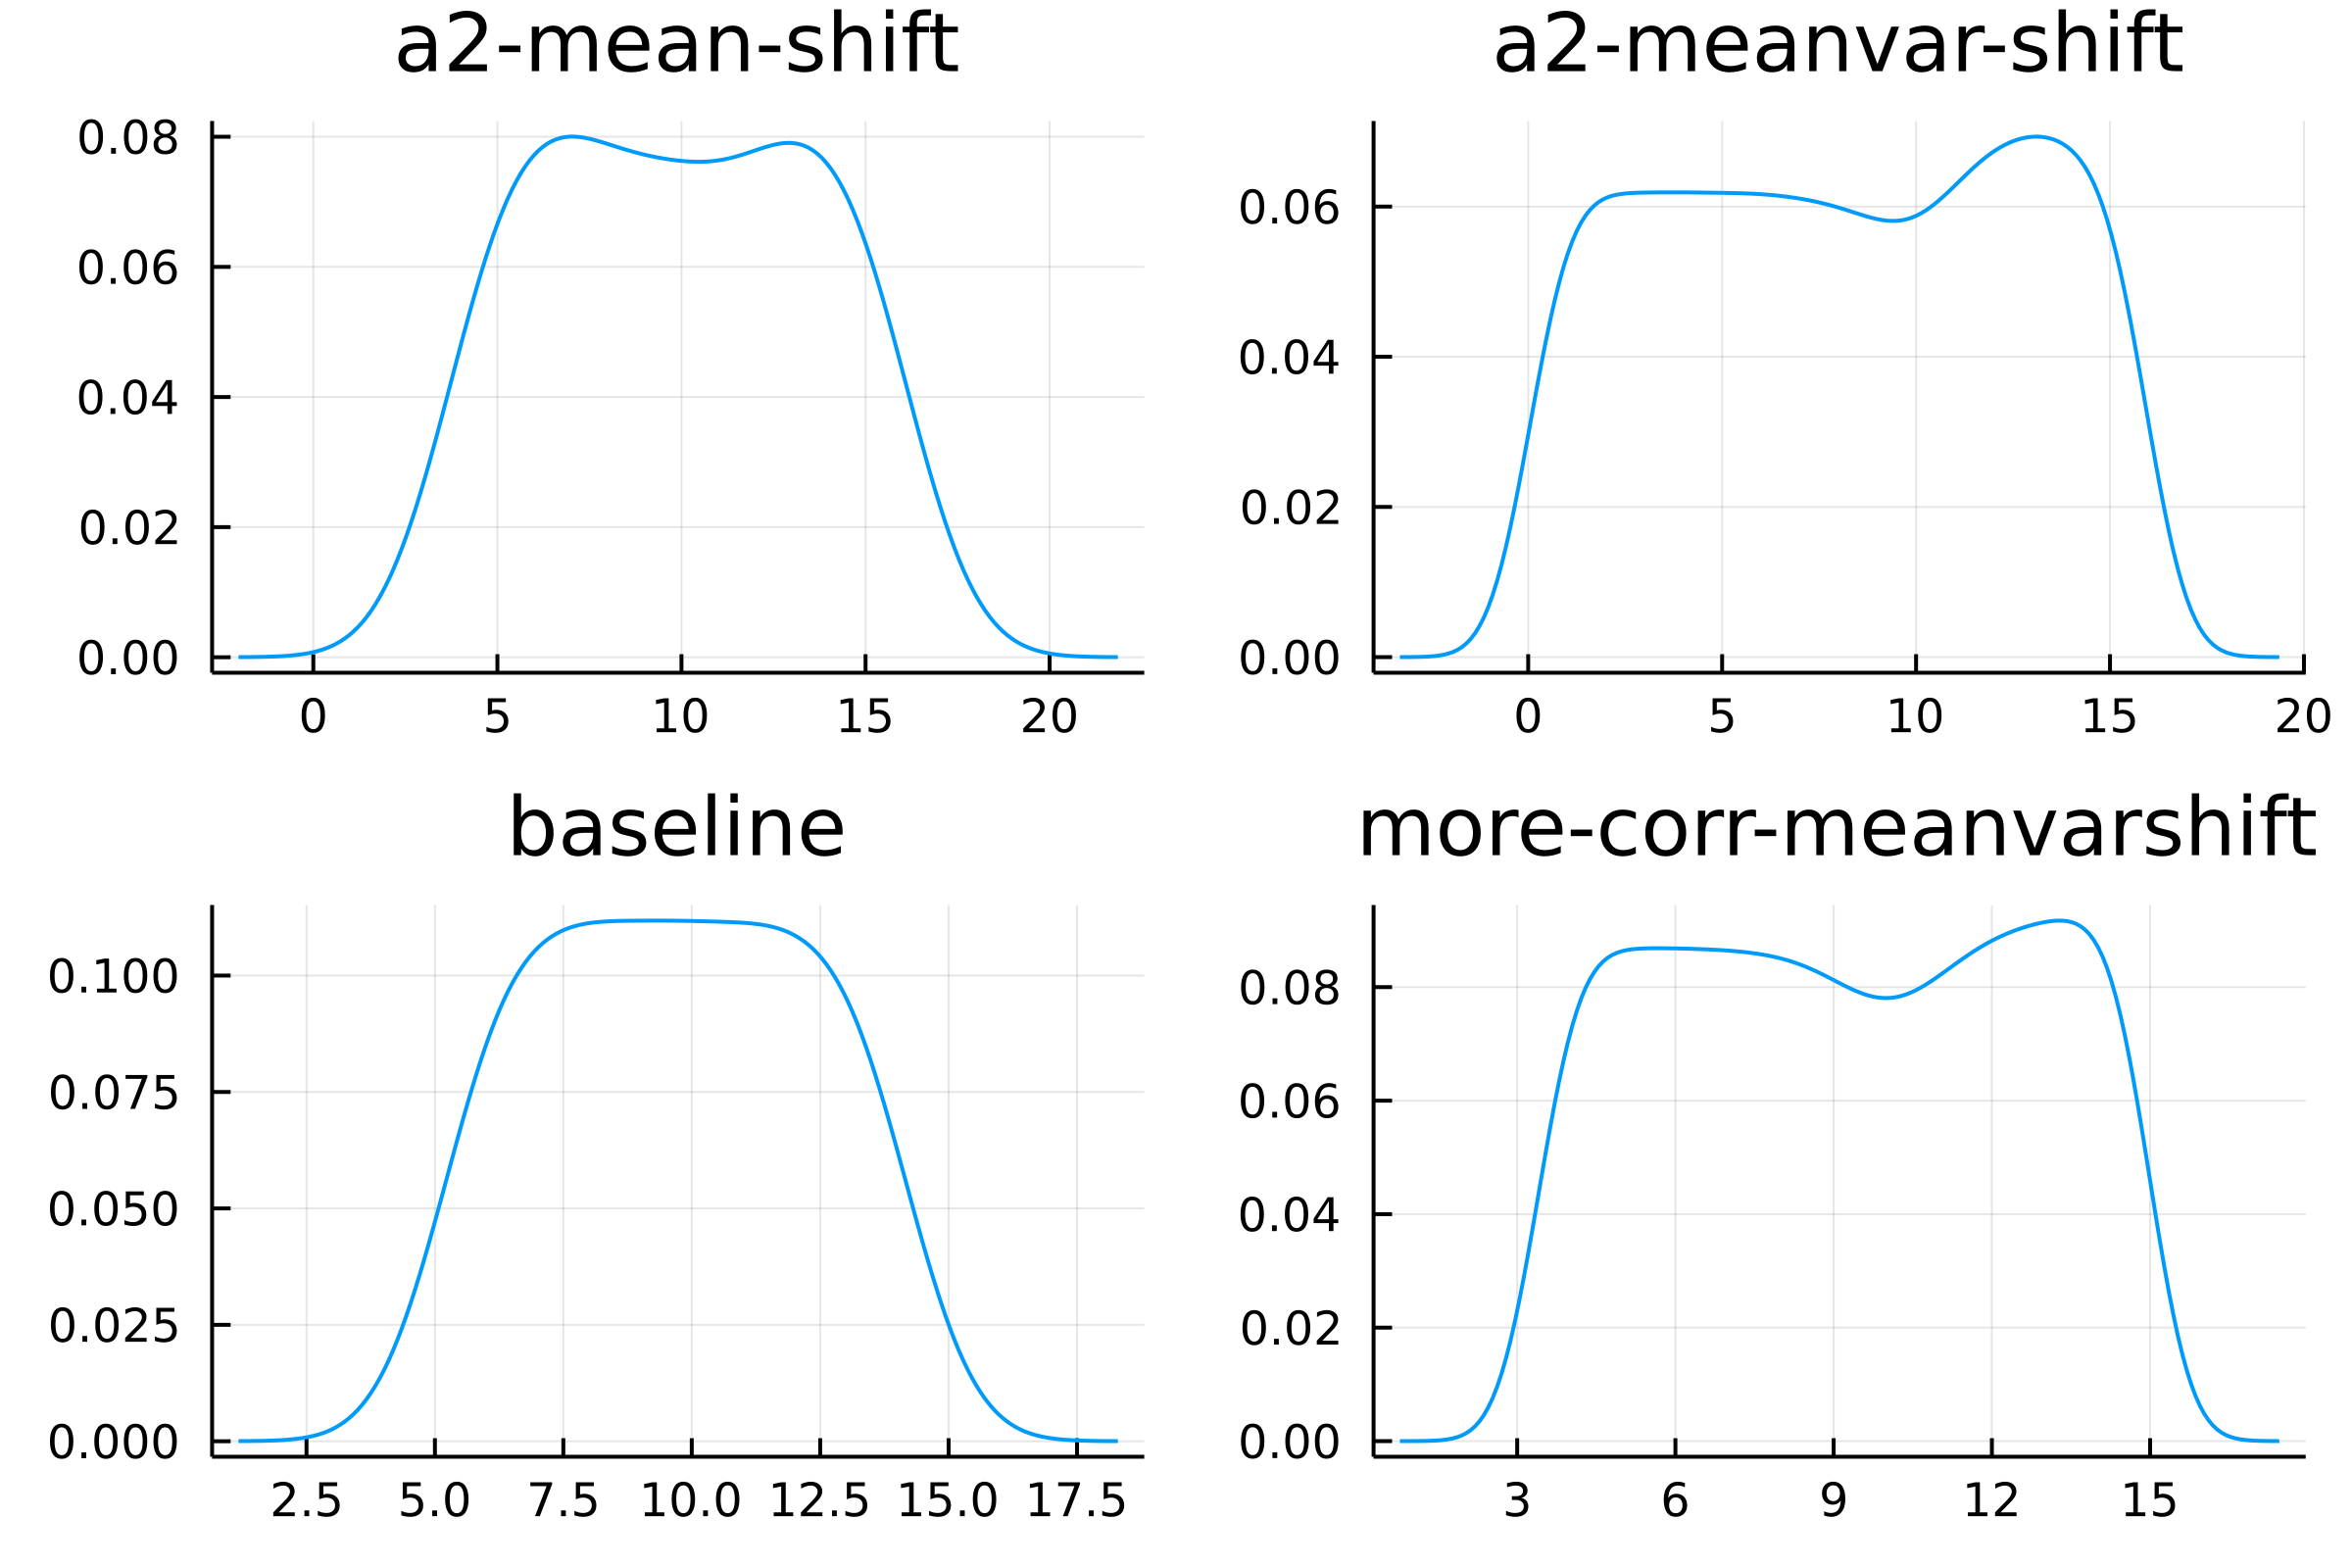
\includegraphics[width=0.95\paperheight]{complexity_files/figure-beamer/unnamed-chunk-24-1} \end{center}

\[
\begin{bmatrix}
 \red{p_1} \\ p_2
\end{bmatrix} =
\begin{bmatrix}
 {a_1} \\ a_2
\end{bmatrix}
 + 
 \begin{bmatrix}
 b_{11} & b_{12} \\
 b_{21} & b_{22}
\end{bmatrix}
\begin{bmatrix}
 f_1 \\ f_2
\end{bmatrix}
+
 \begin{bmatrix}
 c_{11} & c_{12} \\
 c_{21} & c_{22}
\end{bmatrix}
\begin{bmatrix}
 x_1 \\ x_2
\end{bmatrix}
\]
\end{frame}

\begin{frame}{}
\protect\hypertarget{section-3}{}
\begin{center}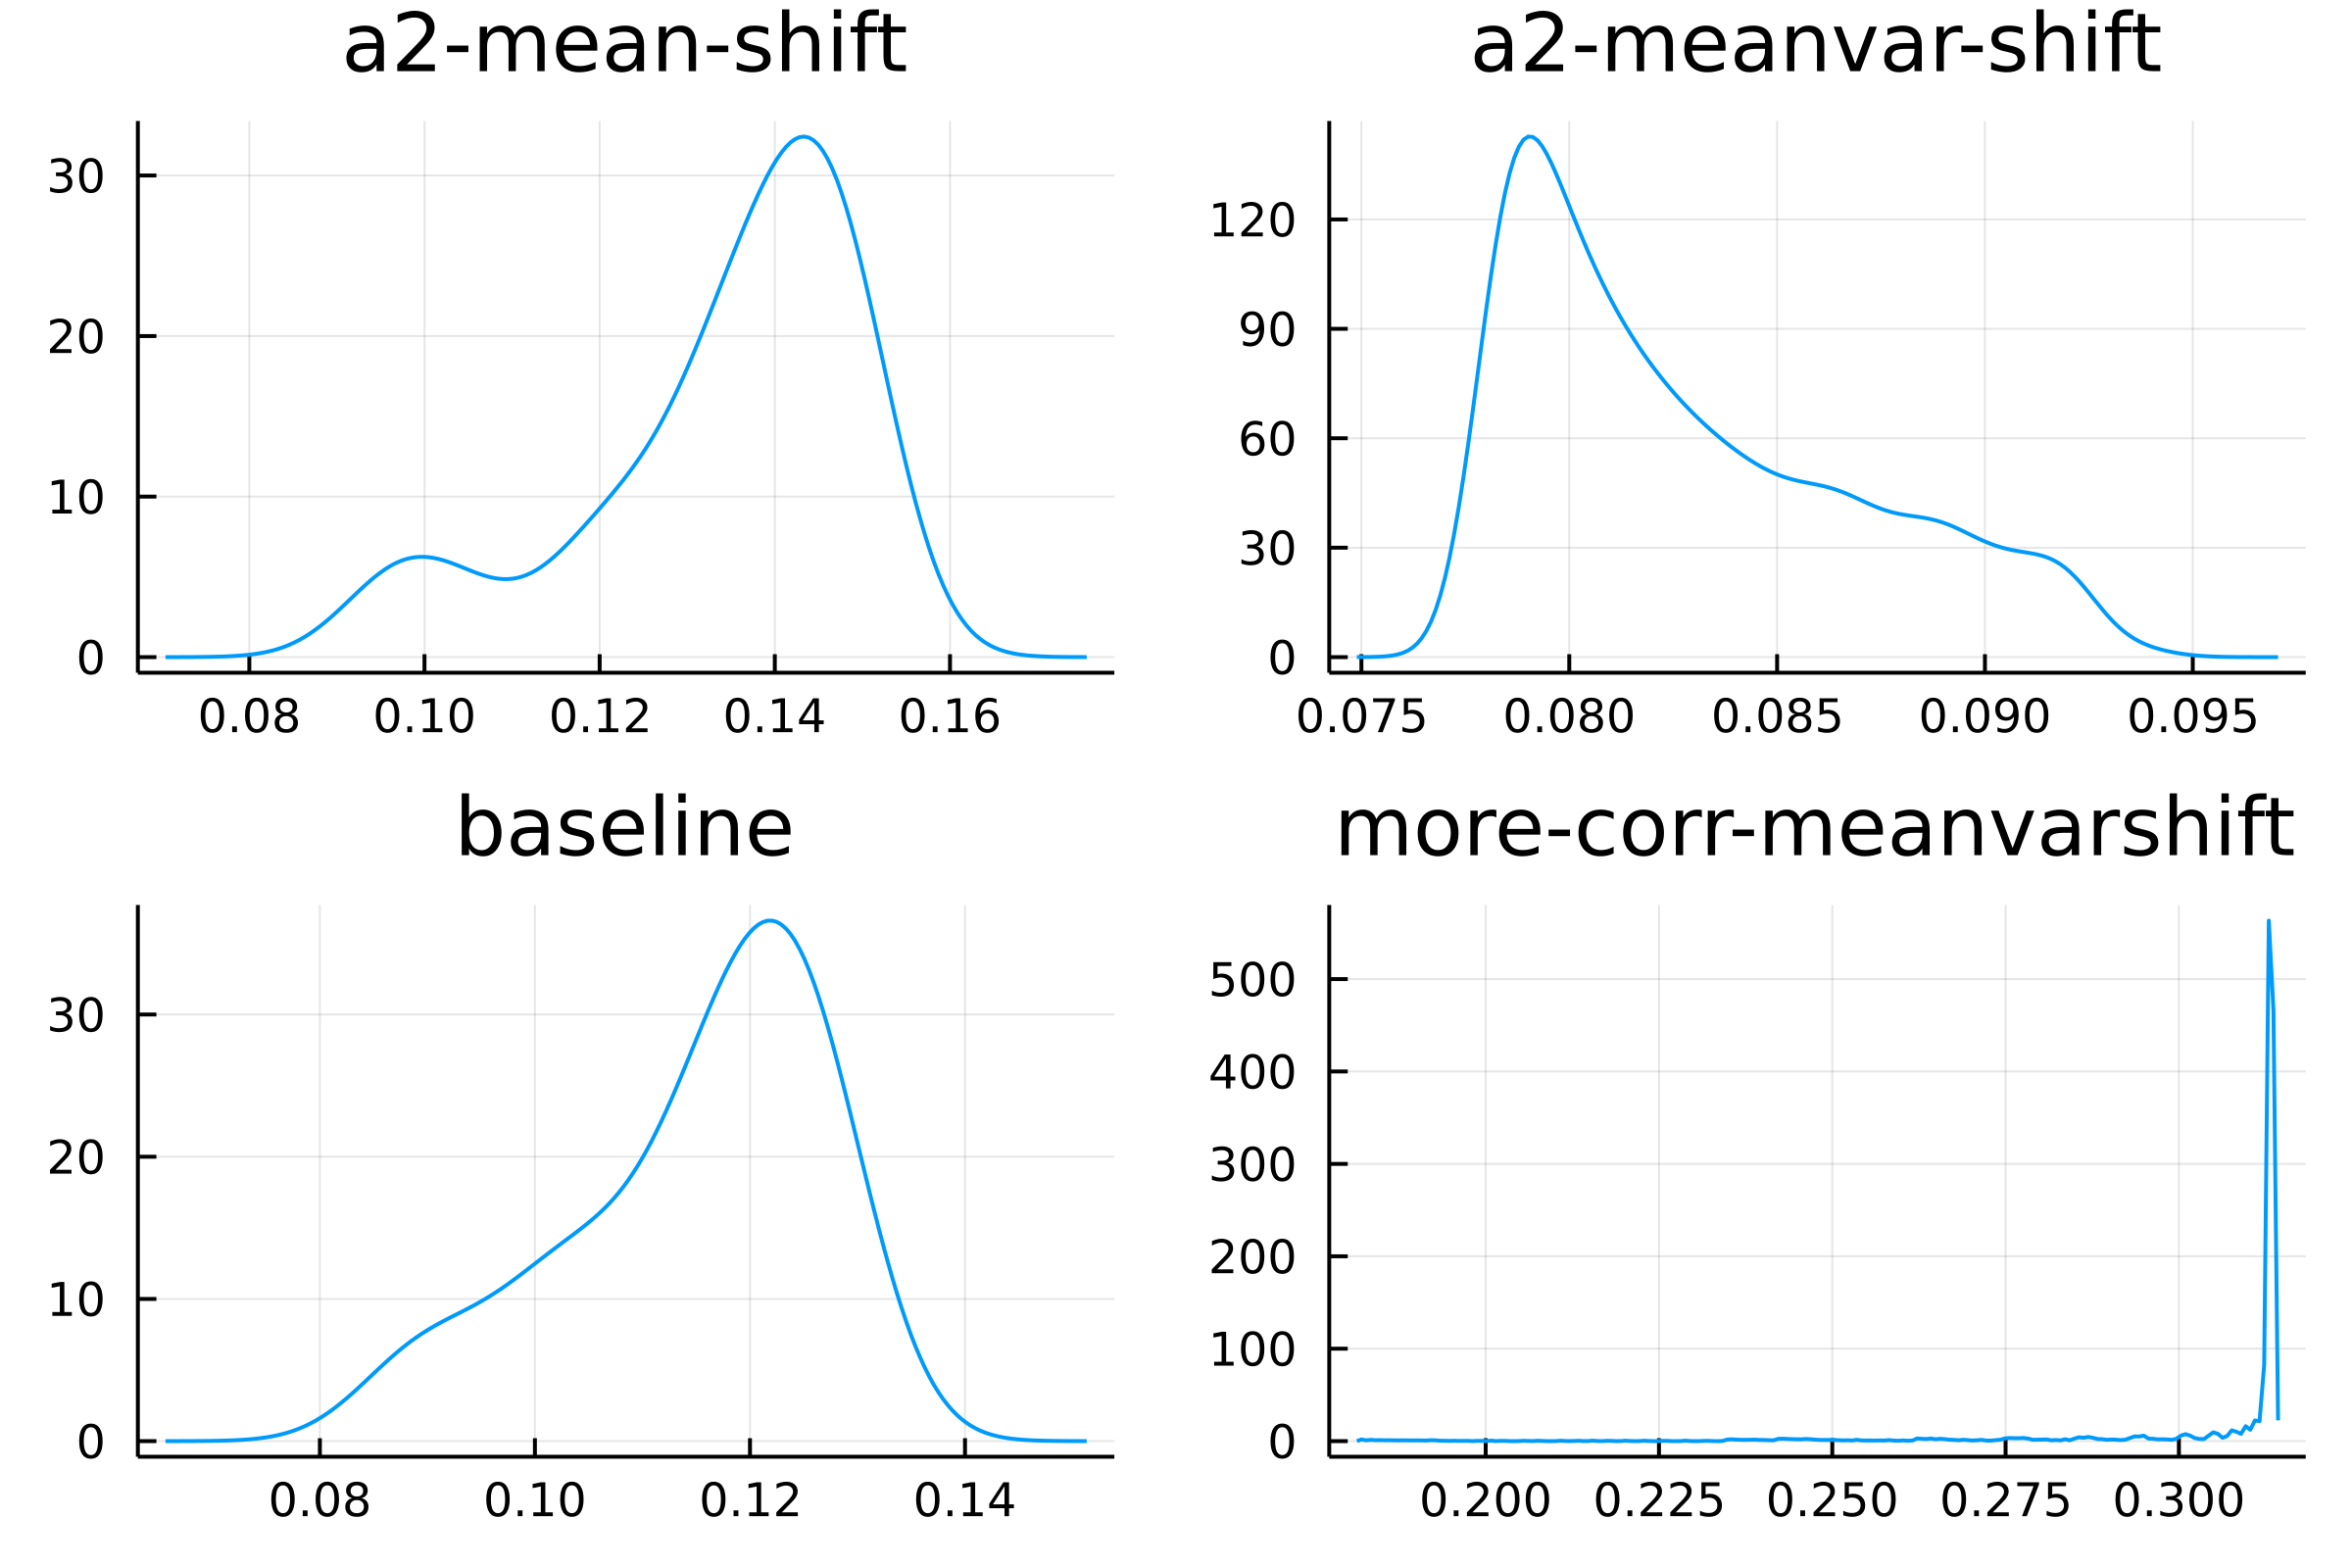
\includegraphics[width=0.95\paperheight]{complexity_files/figure-beamer/unnamed-chunk-25-1} \end{center}

\[
\begin{bmatrix}
 p_1 \\ \red{p_2}
\end{bmatrix} =
\begin{bmatrix}
 {a_1} \\ a_2
\end{bmatrix}
 + 
 \begin{bmatrix}
 b_{11} & b_{12} \\
 b_{21} & b_{22}
\end{bmatrix}
\begin{bmatrix}
 f_1 \\ f_2
\end{bmatrix}
+
 \begin{bmatrix}
 c_{11} & c_{12} \\
 c_{21} & c_{22}
\end{bmatrix}
\begin{bmatrix}
 x_1 \\ x_2
\end{bmatrix}
\]
\end{frame}

\begin{frame}{}
\protect\hypertarget{section-4}{}
\begin{center}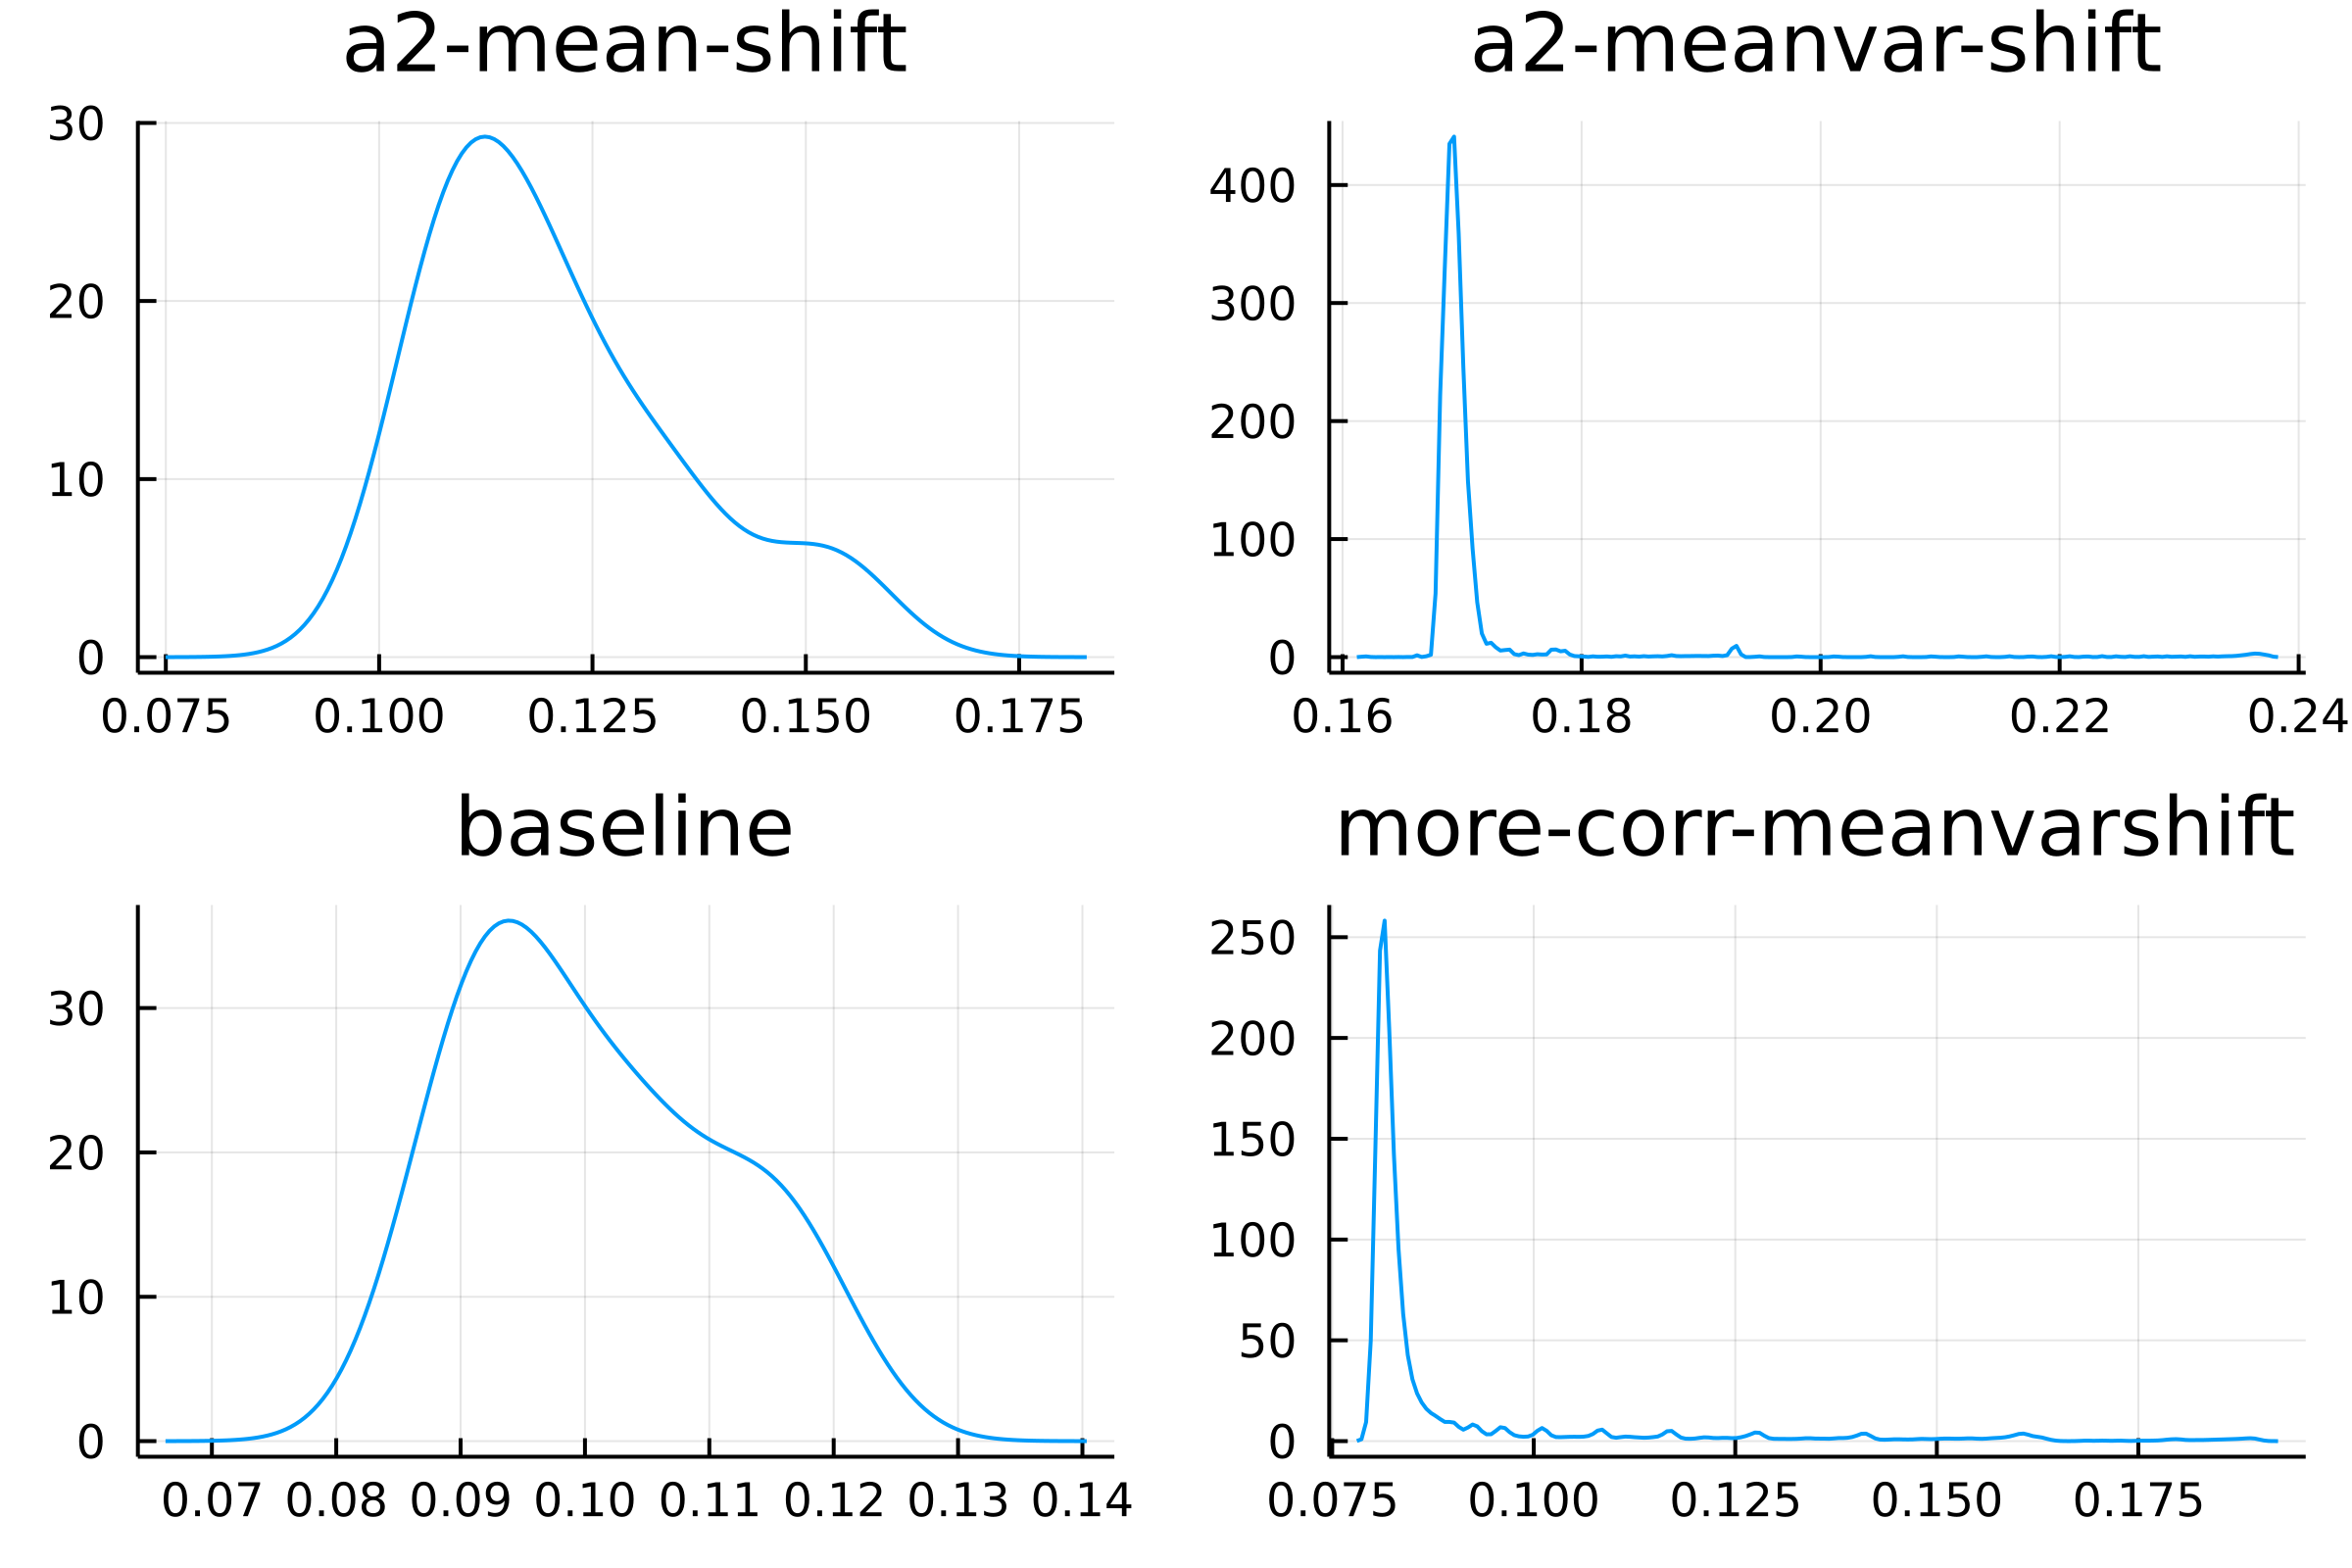
\includegraphics[width=0.95\paperheight]{complexity_files/figure-beamer/unnamed-chunk-26-1} \end{center}

\[
\begin{bmatrix}
 p_1 \\ p_2
\end{bmatrix} =
\begin{bmatrix}
 \red{a_1} \\ a_2
\end{bmatrix}
 + 
 \begin{bmatrix}
 b_{11} & b_{12} \\
 b_{21} & b_{22}
\end{bmatrix}
\begin{bmatrix}
 f_1 \\ f_2
\end{bmatrix}
+
 \begin{bmatrix}
 c_{11} & c_{12} \\
 c_{21} & c_{22}
\end{bmatrix}
\begin{bmatrix}
 x_1 \\ x_2
\end{bmatrix}
\]
\end{frame}

\begin{frame}{}
\protect\hypertarget{section-5}{}
\begin{center}\includegraphics[width=0.95\paperheight]{complexity_files/figure-beamer/unnamed-chunk-27-1} \end{center}

\[
\begin{bmatrix}
 p_1 \\ p_2
\end{bmatrix} =
\begin{bmatrix}
 a_1 \\ \red{a_2}
\end{bmatrix}
 + 
 \begin{bmatrix}
 b_{11} & b_{12} \\
 b_{21} & b_{22}
\end{bmatrix}
\begin{bmatrix}
 f_1 \\ f_2
\end{bmatrix}
+
 \begin{bmatrix}
 c_{11} & c_{12} \\
 c_{21} & c_{22}
\end{bmatrix}
\begin{bmatrix}
 x_1 \\ x_2
\end{bmatrix}
\]
\end{frame}

\begin{frame}{}
\protect\hypertarget{section-6}{}
\begin{center}\includegraphics[width=0.95\paperheight]{complexity_files/figure-beamer/unnamed-chunk-28-1} \end{center}

\[
\begin{bmatrix}
 p_1 \\ p_2
\end{bmatrix} =
\begin{bmatrix}
 a_1 \\ {a_2}
\end{bmatrix}
 + 
 \begin{bmatrix}
 \red{b_{11}} & b_{12} \\
 b_{21} & b_{22}
\end{bmatrix}
\begin{bmatrix}
 f_1 \\ f_2
\end{bmatrix}
+
 \begin{bmatrix}
 c_{11} & c_{12} \\
 c_{21} & c_{22}
\end{bmatrix}
\begin{bmatrix}
 x_1 \\ x_2
\end{bmatrix}
\]
\end{frame}

\begin{frame}{}
\protect\hypertarget{section-7}{}
\begin{center}\includegraphics[width=0.95\paperheight]{complexity_files/figure-beamer/unnamed-chunk-29-1} \end{center}

\[
\begin{bmatrix}
 p_1 \\ p_2
\end{bmatrix} =
\begin{bmatrix}
 a_1 \\ {a_2}
\end{bmatrix}
 + 
 \begin{bmatrix}
 {b_{11}} & b_{12} \\
 b_{21} & \red{b_{22}}
\end{bmatrix}
\begin{bmatrix}
 f_1 \\ f_2
\end{bmatrix}
+
 \begin{bmatrix}
 c_{11} & c_{12} \\
 c_{21} & c_{22}
\end{bmatrix}
\begin{bmatrix}
 x_1 \\ x_2
\end{bmatrix}
\]
\end{frame}

\begin{frame}{}
\protect\hypertarget{section-8}{}
\begin{center}\includegraphics[width=0.95\paperheight]{complexity_files/figure-beamer/unnamed-chunk-30-1} \end{center}

\[
\begin{bmatrix}
 p_1 \\ p_2
\end{bmatrix} =
\begin{bmatrix}
 a_1 \\ {a_2}
\end{bmatrix}
 + 
 \begin{bmatrix}
 {b_{11}} & \red{b_{12}} \\
 {b_{21}} & {b_{22}}
\end{bmatrix}
\begin{bmatrix}
 f_1 \\ f_2
\end{bmatrix}
+
 \begin{bmatrix}
 c_{11} & c_{12} \\
 c_{21} & c_{22}
\end{bmatrix}
\begin{bmatrix}
 x_1 \\ x_2
\end{bmatrix}
\]
\end{frame}

\begin{frame}{}
\protect\hypertarget{section-9}{}
\begin{center}\includegraphics[width=0.95\paperheight]{complexity_files/figure-beamer/unnamed-chunk-31-1} \end{center}

\[
\begin{bmatrix}
 p_1 \\ p_2
\end{bmatrix} =
\begin{bmatrix}
 a_1 \\ {a_2}
\end{bmatrix}
 + 
 \begin{bmatrix}
 {b_{11}} & b_{12} \\
 {b_{21}} & {b_{22}}
\end{bmatrix}
\begin{bmatrix}
 f_1 \\ f_2
\end{bmatrix}
+
 \begin{bmatrix}
 \red{c_{11}} & c_{12} \\
 c_{21} & c_{22}
\end{bmatrix}
\begin{bmatrix}
 x_1 \\ x_2
\end{bmatrix}
\]
\end{frame}

\begin{frame}{}
\protect\hypertarget{section-10}{}
\begin{center}\includegraphics[width=0.95\paperheight]{complexity_files/figure-beamer/unnamed-chunk-32-1} \end{center}

\[
\begin{bmatrix}
 p_1 \\ p_2
\end{bmatrix} =
\begin{bmatrix}
 a_1 \\ {a_2}
\end{bmatrix}
 + 
 \begin{bmatrix}
 {b_{11}} & b_{12} \\
 {b_{21}} & {b_{22}}
\end{bmatrix}
\begin{bmatrix}
 f_1 \\ f_2
\end{bmatrix}
+
 \begin{bmatrix}
 {c_{11}} & c_{12} \\
 c_{21} & \red{c_{22}}
\end{bmatrix} 
\begin{bmatrix}
 x_1 \\ x_2
\end{bmatrix}
\]
\end{frame}

\begin{frame}{}
\protect\hypertarget{section-11}{}
\begin{center}\includegraphics[width=0.95\paperheight]{complexity_files/figure-beamer/unnamed-chunk-33-1} \end{center}

\[
\begin{bmatrix}
 p_1 \\ p_2
\end{bmatrix} =
\begin{bmatrix}
 a_1 \\ {a_2}
\end{bmatrix}
 + 
 \begin{bmatrix}
 {b_{11}} & b_{12} \\
 {b_{21}} & {b_{22}}
\end{bmatrix}
\begin{bmatrix}
 f_1 \\ f_2
\end{bmatrix}
+
 \begin{bmatrix}
 {c_{11}} & \red{c_{12}} \\
 c_{21} & {c_{22}}
\end{bmatrix} 
\begin{bmatrix}
 x_1 \\ x_2
\end{bmatrix}
\]
\end{frame}

\hypertarget{next-steps}{%
\section{Next steps}\label{next-steps}}

\begin{frame}{Next steps}
\protect\hypertarget{next-steps-1}{}
\begin{enumerate}
\tightlist
\item
  Solve the ex-ante information choice problem.
\item
  Solve the hidden attention allocation modification, a mixed strategy
  on \(\Sigma_{\eta_j}\).
\item
  Estimate the (observed) joint density (\(f\)) of many assets. Which
  assets should we see the most attention on given my understanding of
  \(\Sigma_{\eta_j}(\mathbf{\mu}, \mathbf{\Sigma})\)?
\end{enumerate}
\end{frame}

\end{document}
